\documentclass{beamer}
\usetheme{Singapore}
%\setbeamercolor{structure}{fg=red}
\usepackage{upgreek}
\usepackage{color}
%\def\magyarOptions{hyphenation=huhyphn}
%\usepackage{ae,aecompl}
%\usepackage[T1]{fontenc}
\usepackage[utf8]{inputenc}
%\usepackage[hungarian]{babel}
\usepackage{gensymb}
\usepackage{tikz}
\usepackage[framemethod=tikz]{mdframed}
\usepackage[version=3]{mhchem}


\normalfont
\title{Recent Advances in Potentiometric Scanning Electrochemical Microscopy}
\author
{author:\\
András Kiss\\
\hfill \\
supervisor:\\
prof. Géza Nagy}

\institute
{
  %\inst{1}%
  Department of General and Physical Chemistry\\
  University of Pécs, Hungary\\
  \hfill \\

  
\includegraphics[width=0.14\textwidth]{pte_logo.eps}\\
  April 18, 2017
}

\date[]

\begin{document}
\frame{\titlepage}  


\begin{frame}
	\centering
	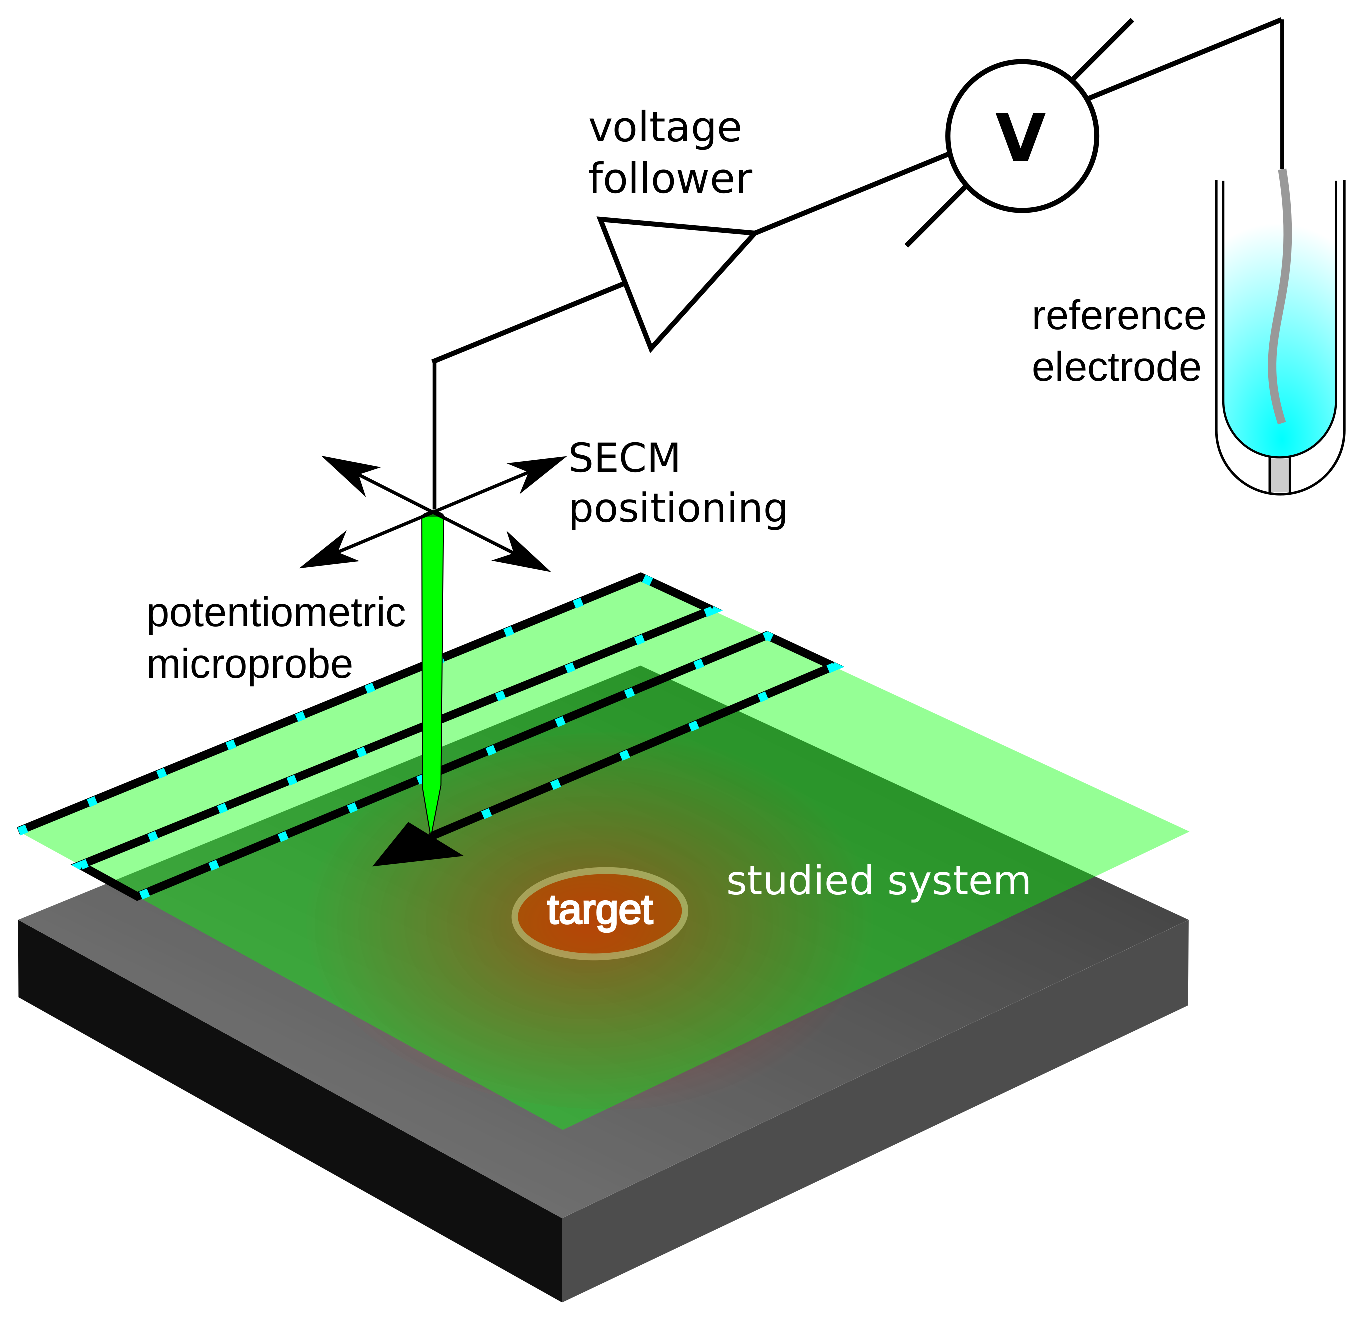
\includegraphics[width=0.6\textwidth]{secm.eps}
	\frametitle{Potentiometric Scanning Electrochemical Microscopy}
	\framesubtitle{A Scanning Probe Microscopic technique}

\end{frame}


\begin{frame}
\frametitle{Ion-selective micropipettes}
\framesubtitle{As SECM probes}
\begin{columns}[T] % align columns
\begin{column}{.48\textwidth}

\centering
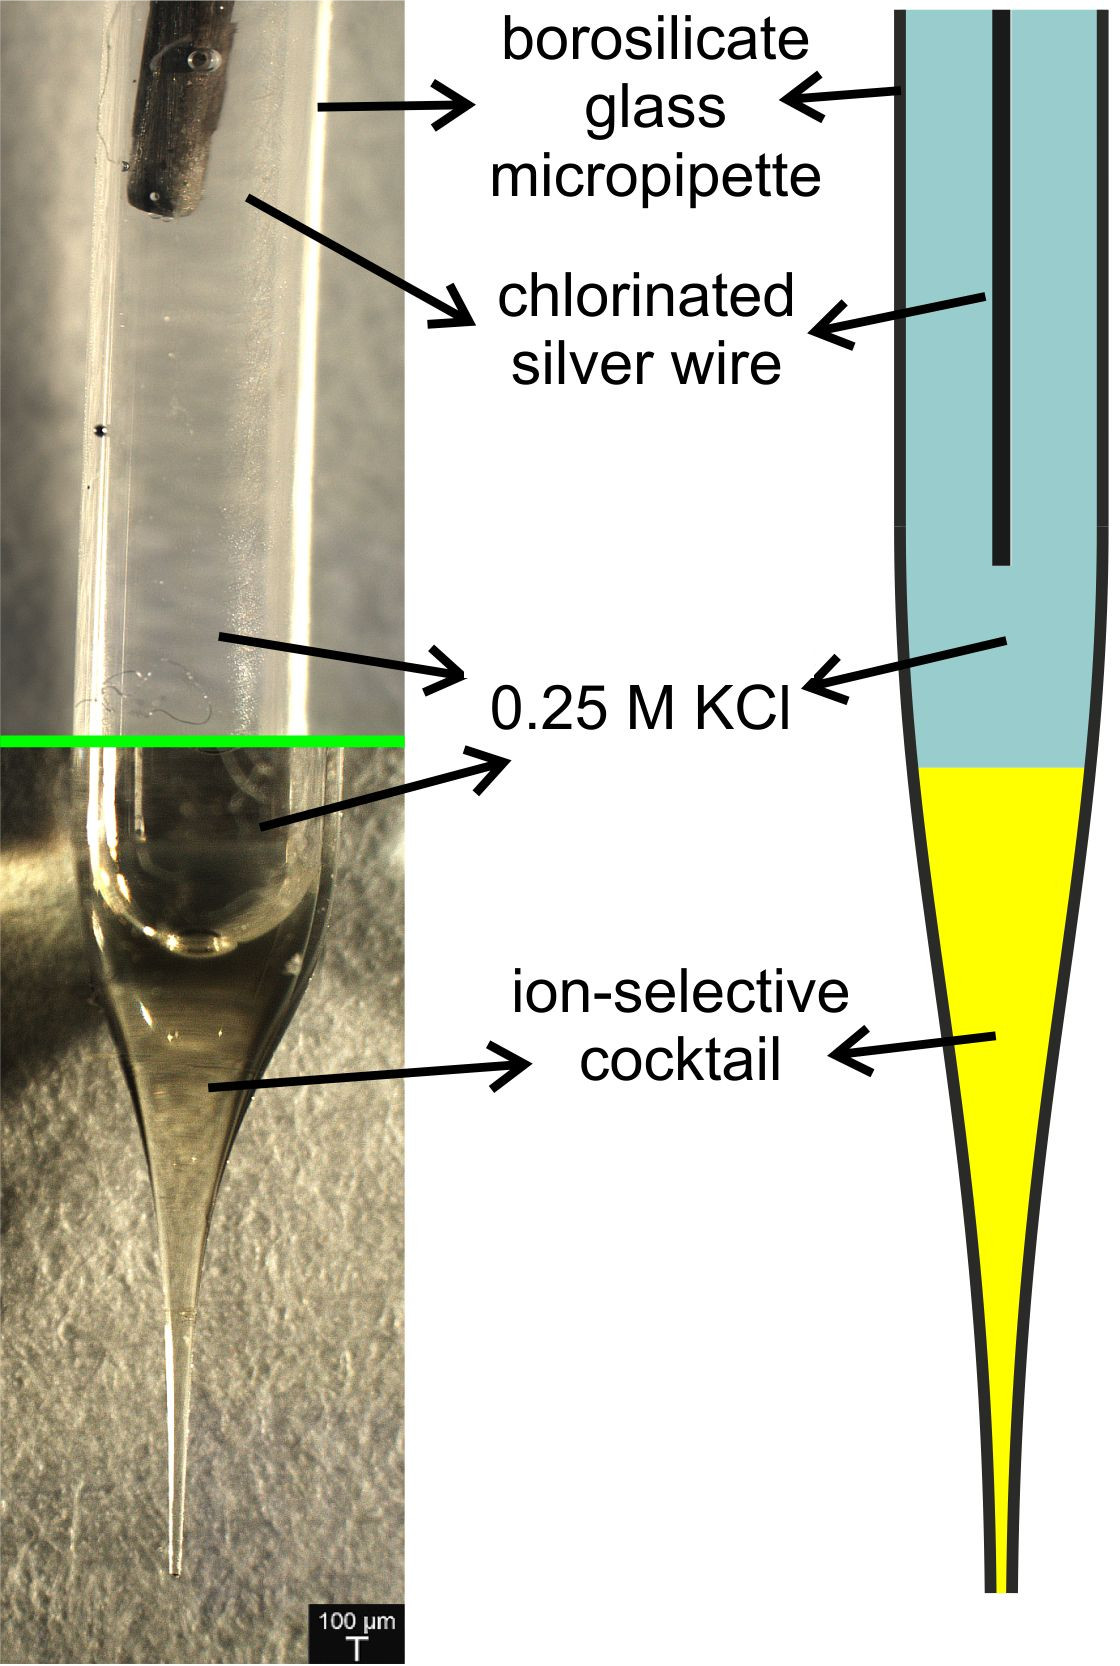
\includegraphics[width=0.9\textwidth]{liquid.jpg}
\end{column}%
\hfill%
\begin{column}{.48\textwidth}
%\color{blue}\rule{\linewidth}{4pt}
\centering

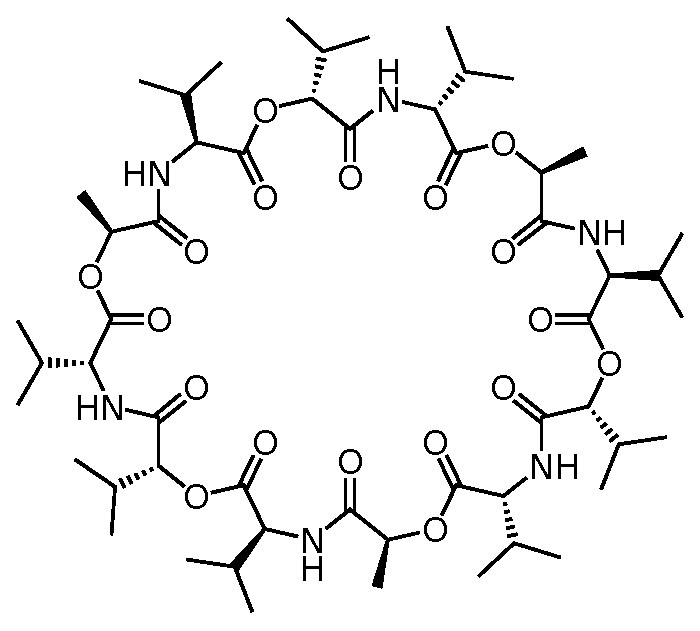
\includegraphics[width=0.8\textwidth]{Valinomycin.eps}

Valinomycin
\vfill

\footnotesize
\begin{equation*}
        E=E^\theta + \frac{RT}{z_iF} \ln \left [ a_i + \sum_{j} \left ( k_{ij}a_j^{z_i/z_j} \right ) \right ]
        \end{equation*}
\normalsize
Nikolsky--equation
\end{column}%
\end{columns}
\end{frame}

\begin{frame}
	\frametitle{The problem with potentiometric SECM} 
	\framesubtitle{Distortion at high scan rate}
	\centering
\quad\quad\quad\quad\quad\quad Slow \hfill Fast \quad\quad\quad\quad\quad\quad\quad

	\includegraphics[trim = 10mm 30mm 0mm 20mm, clip, width=0.4\textwidth, angle=-90]{real.eps}\hfill\includegraphics[trim = 10mm 30mm 0mm 20mm, clip, width=0.4\textwidth, angle=-90]{fastcomb_sim.eps}
\end{frame}

\begin{frame}
	\frametitle{Why is the image distorted?}
	\framesubtitle{The RC time constant} 
	\centering
	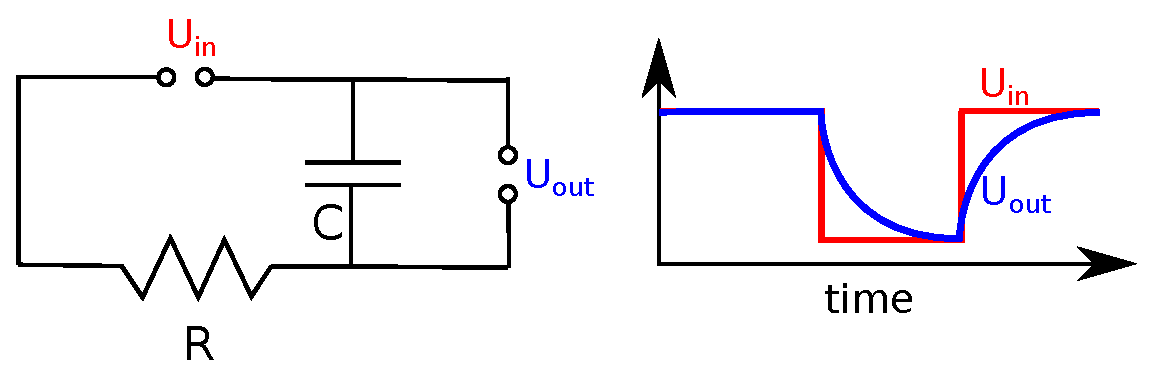
\includegraphics[width=1\textwidth]{RC.eps}
	\vfill
	The time required to discharge the capacitor by $\approx 37\%$ $(1/e)$.
	
	Or to charge it by $\approx 63\%$ $(1-1/e)$.	
	\vfill
	$\tau = R \cdot C$
	
	$R = 5 $ G$\ohm$
	
	$C = 500 $ pF
	
	\textbf{\textcolor{white!100}{\colorbox{red!100}{$\tau = 2.5 $ s}}}

	%\includegraphics[width=0.6\textwidth, angle=-90]{meander_sim.eps}
\end{frame}

\begin{frame}
	\frametitle{Distortion of potentiometric imaging} 
	\framesubtitle{In the case of a linescan} 
	\centering
	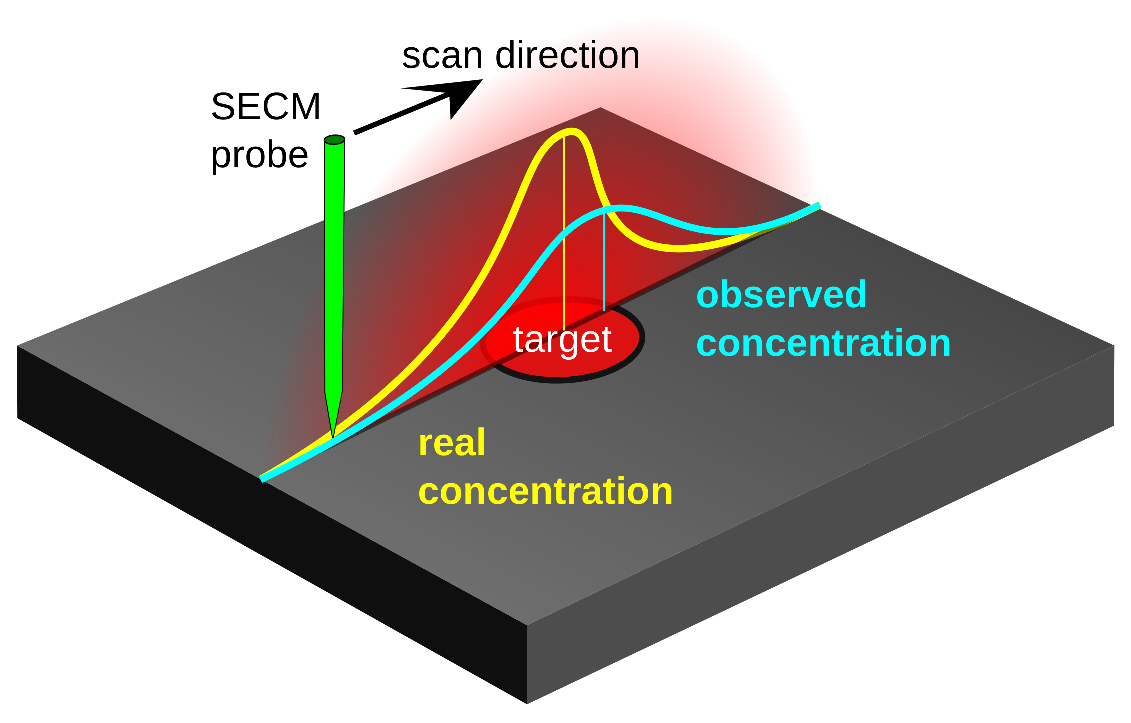
\includegraphics[width=0.8\textwidth]{distortion2.eps}
\end{frame}

\begin{frame}
	\frametitle{Why is it so important to complete the scan quickly?}
	\framesubtitle{Example: corrosion of a magnesium alloy}
	\includegraphics[width=1\textwidth]{timelapse.eps}\\
\centering
Corrosion of the AZ63 magnesium-aluminium-zinc alloy.
%Location of the anodic and cathodic spots change quickly. High-speed scanning is required to complete the scan before the studied system changes.
\end{frame} 

\begin{frame}
\frametitle{Trade-off triangle of potentiometric SECM}
\framesubtitle{Compromise between the three desired competing properties}
\begin{center}
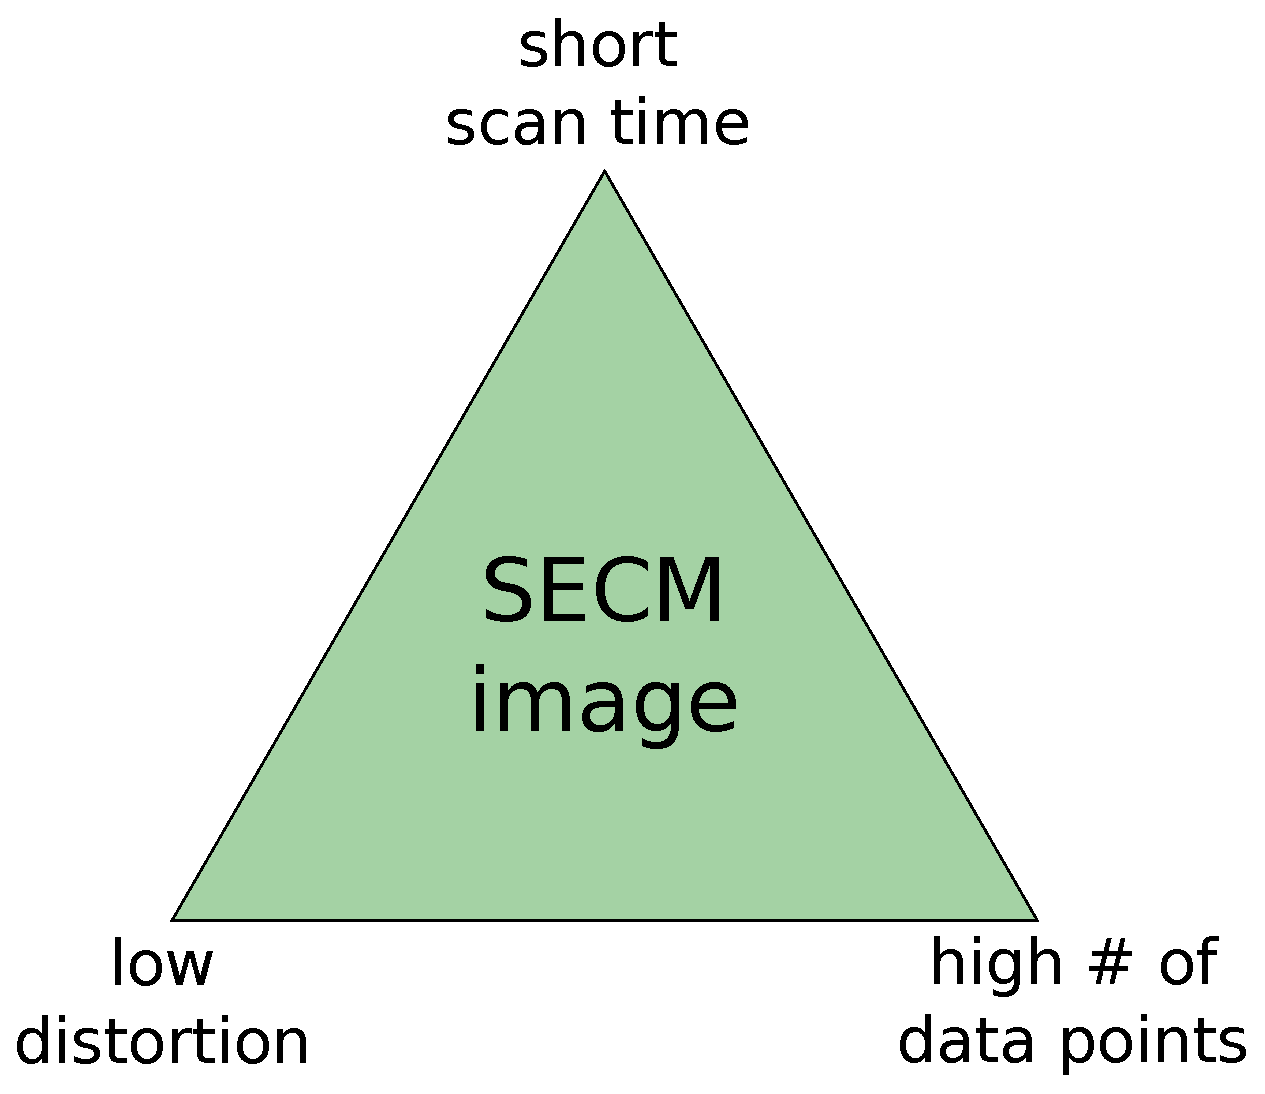
\includegraphics[width=0.5\textwidth]{trade-off.eps}
\end{center}
\end{frame}

\begin{frame}[plain]
\centering
Solution \#1:
Solid contact micropipettes as SECM probes.
\end{frame}

\begin{frame}
\frametitle{Liquid vs. solid contact micropipettes}
\framesubtitle{Comparison of construction}
\begin{center}
\quad\quad\quad\quad Liquid contact \hfill Solid contact \quad\quad\quad\quad

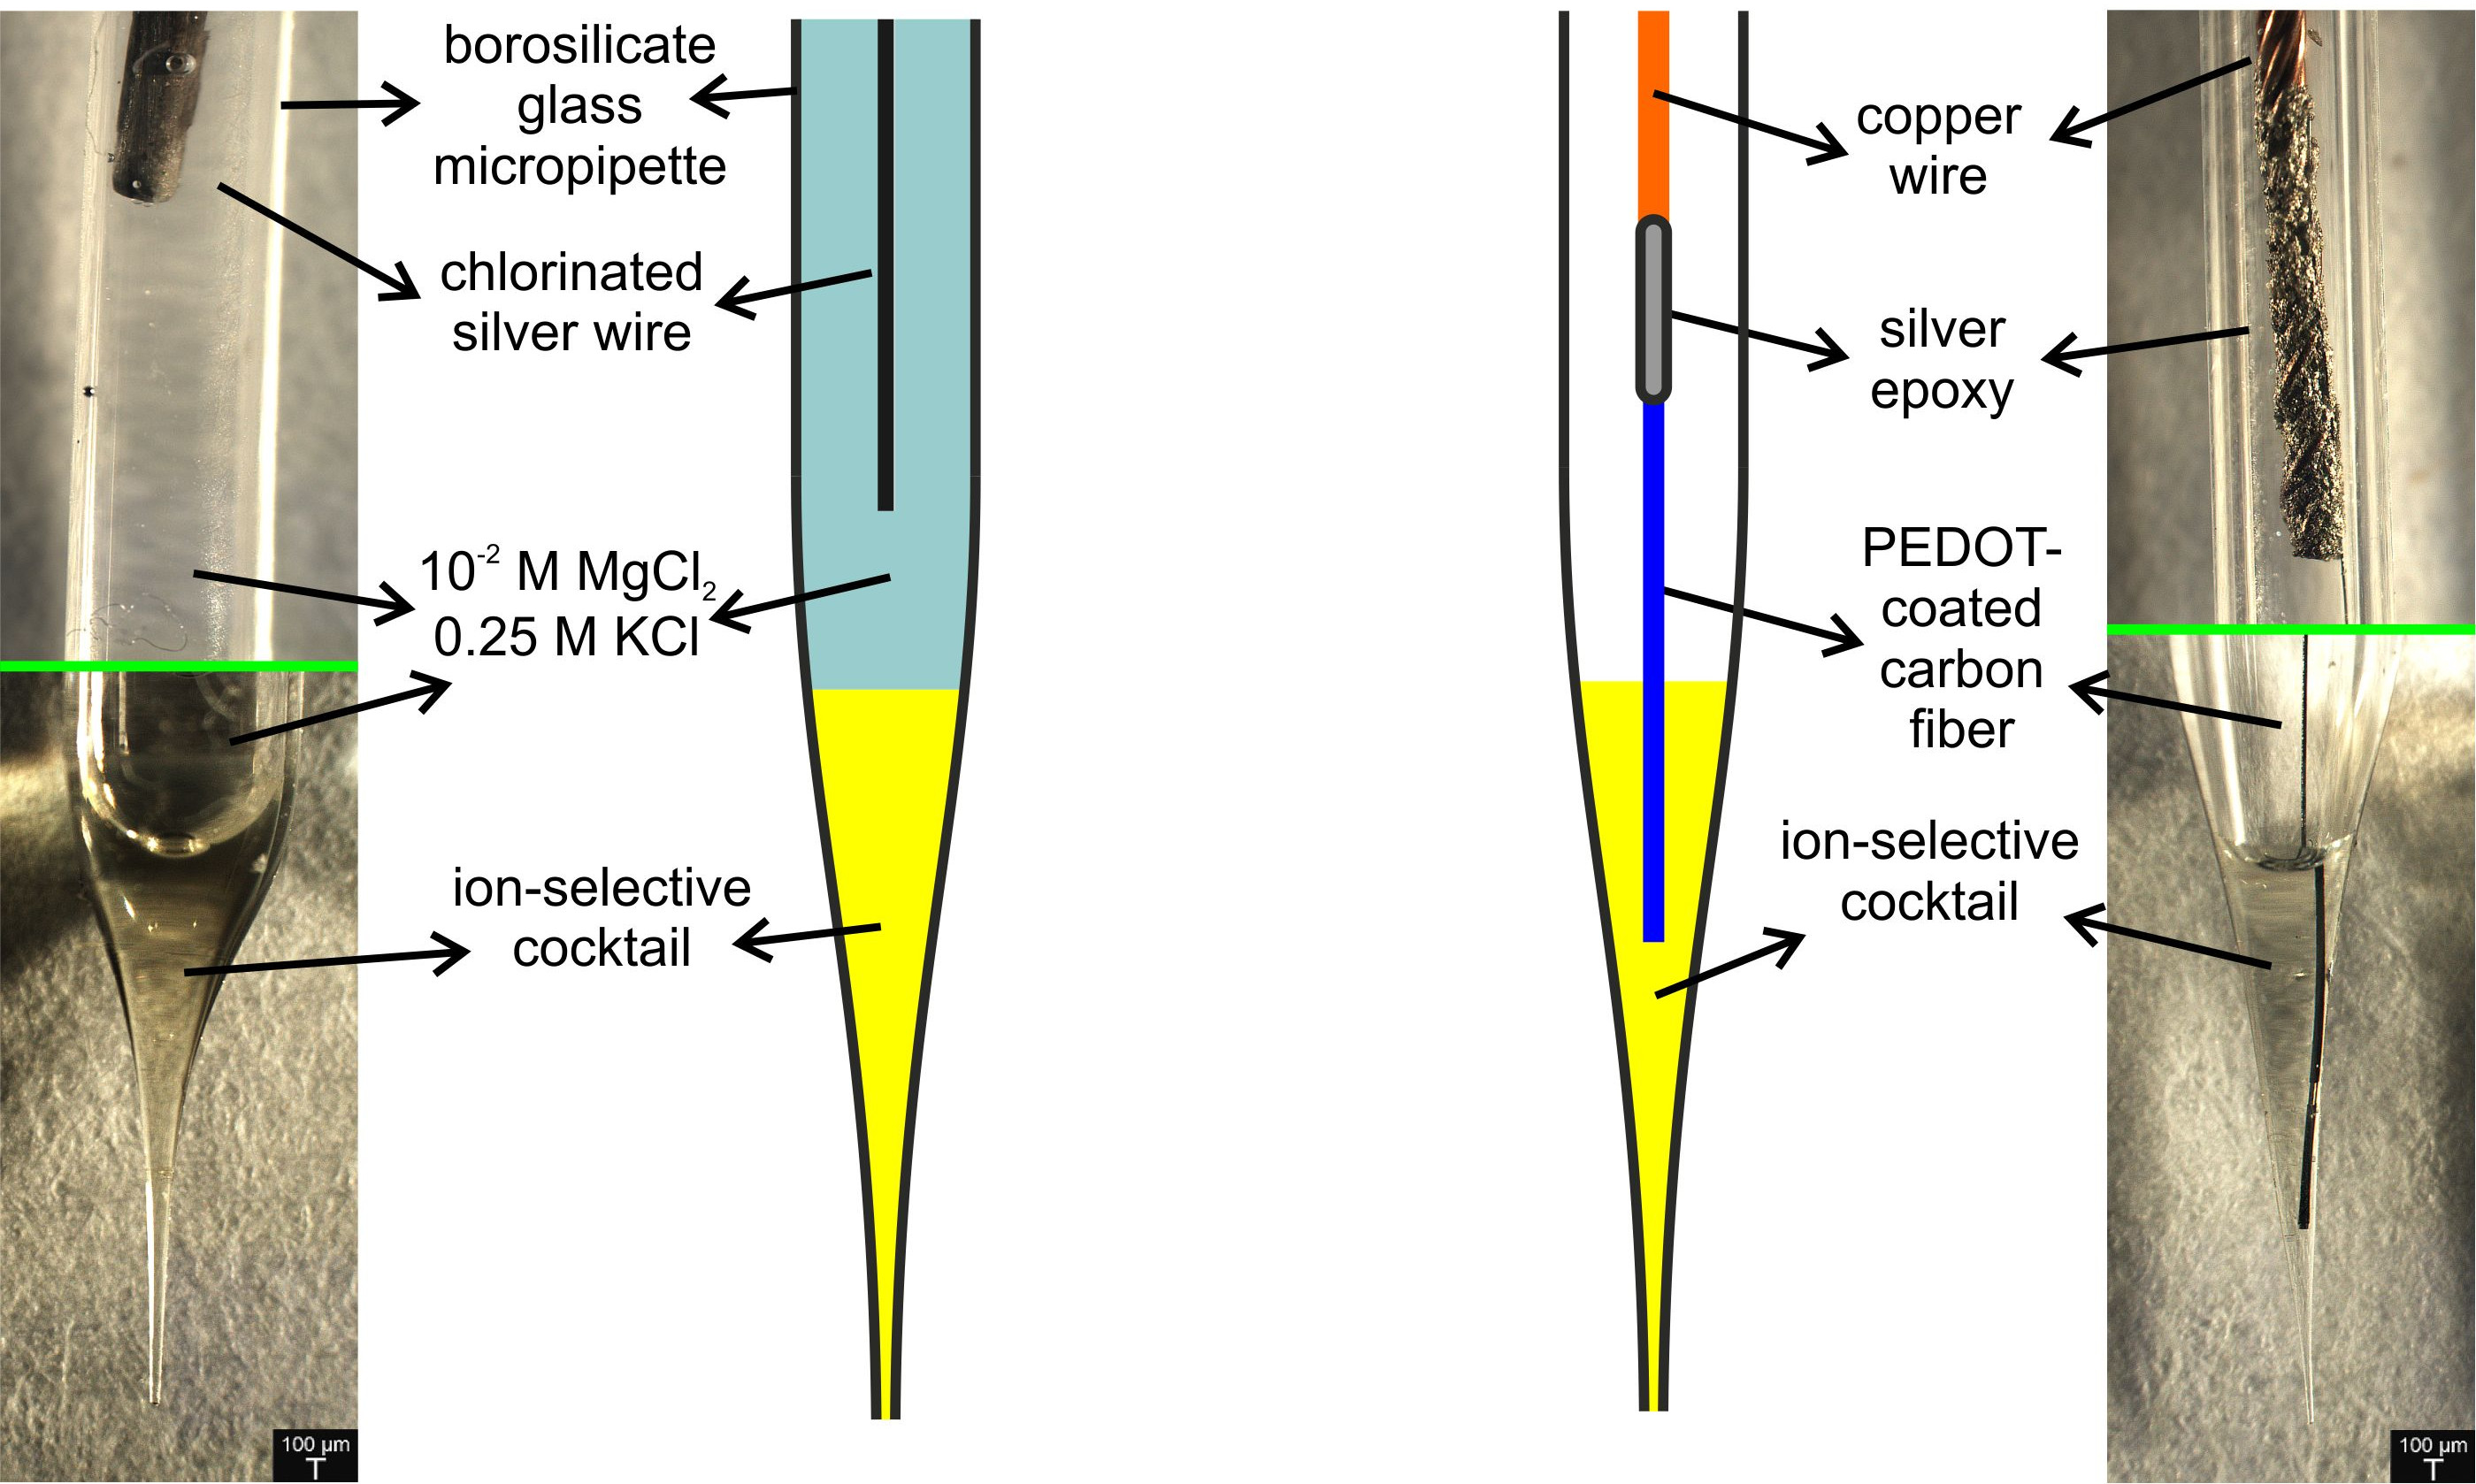
\includegraphics[width=0.9\textwidth]{liquid_solid.jpg}
\end{center}
\end{frame}

\begin{frame}
\frametitle{Comparison of the electrodes' resistance}
\framesubtitle{Voltage divider method and result}
\begin{center}
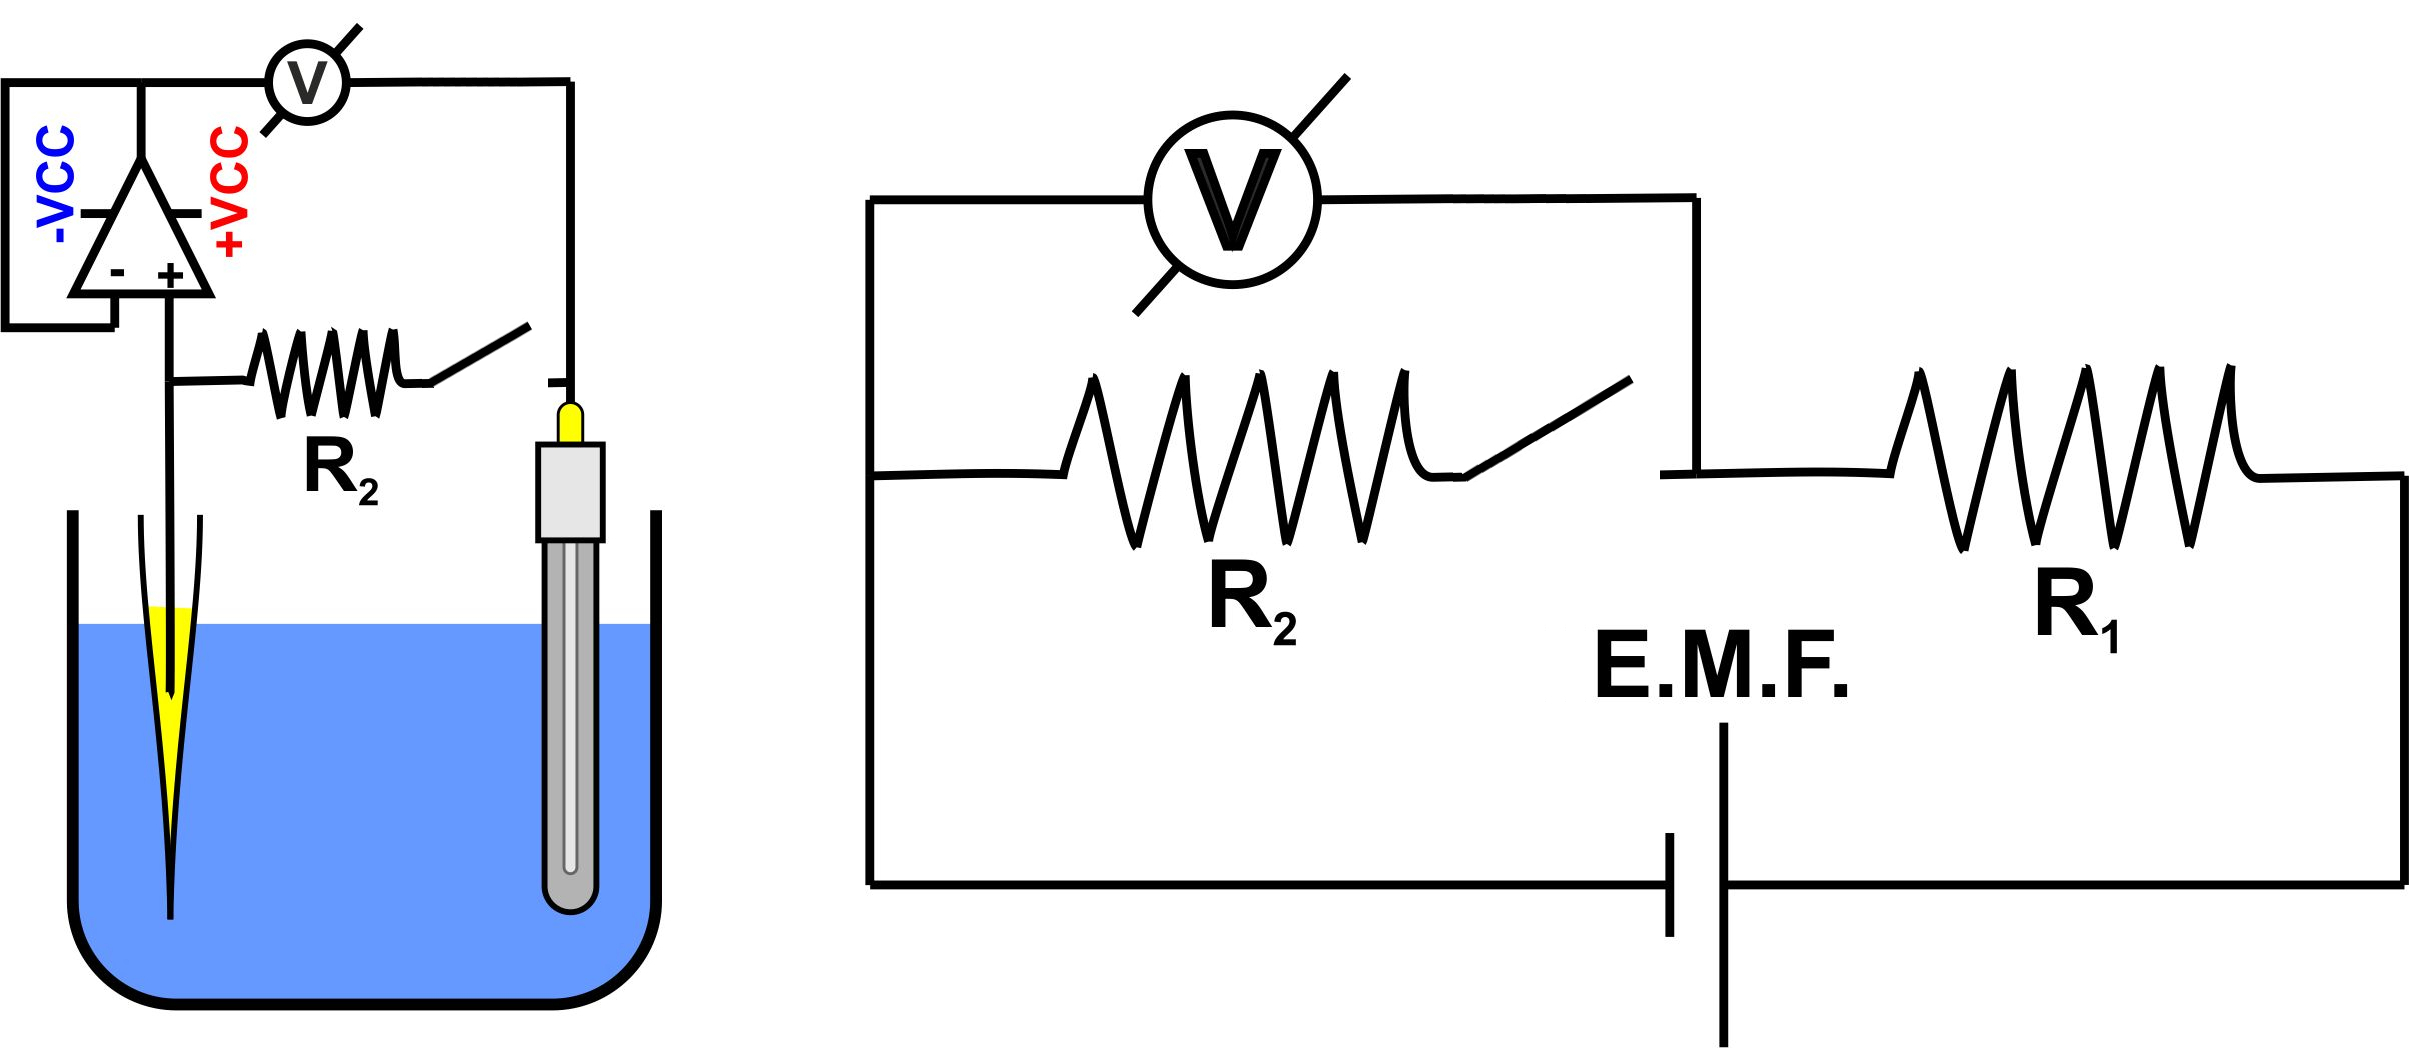
\includegraphics[width=0.7\textwidth]{divider_switch.jpg}
\vfill
\begin{table}
                \centering
                \begin{tabular}{r c}
                        %\hline
                        Type & R$_{ISME}$ / G$\ohm$ \\
			\cline{1-2}
			Liquid contact & \textbf{\textcolor{white!100}{\colorbox{red!100}{4.80}}} \\
                        Solid contact &  \textbf{\textcolor{black!100}{\colorbox{green!100}{0.56}}} \\

                \end{tabular}
\end{table}
\end{center}
\end{frame}

\begin{frame}
\frametitle{Comparison of the electrodes' performance}
\framesubtitle{Experimental setup}
\begin{center}
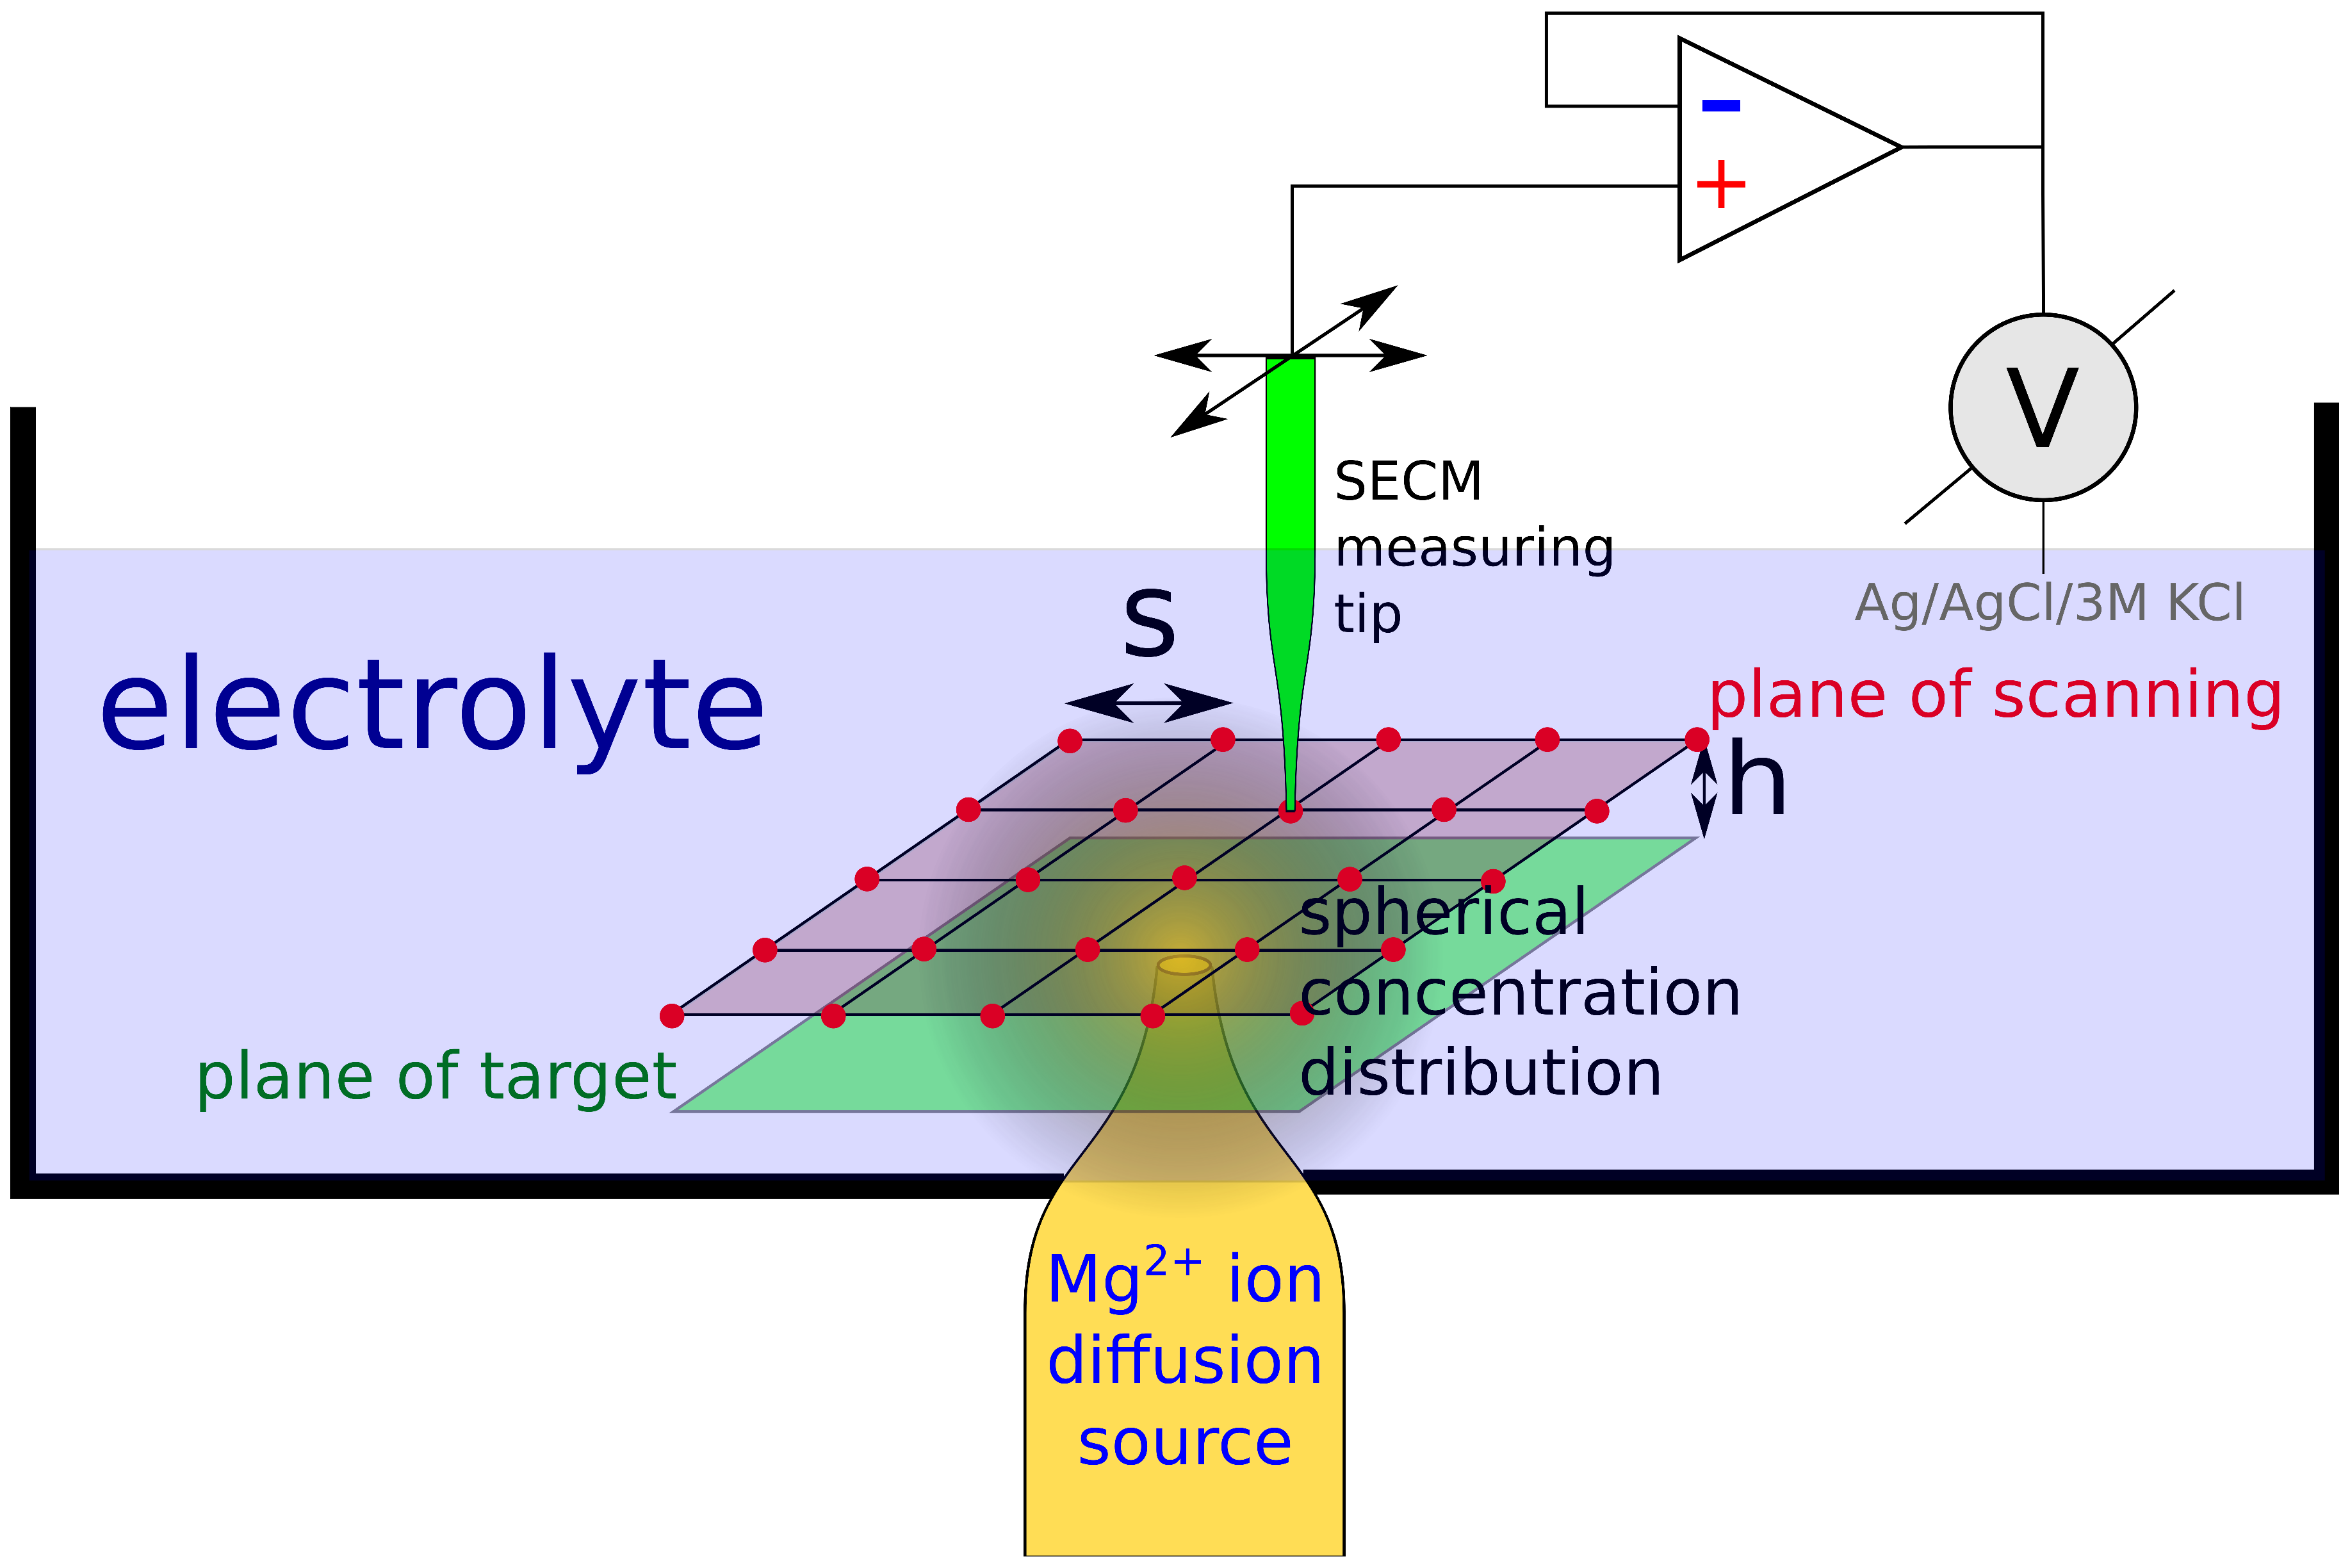
\includegraphics[width=0.9\textwidth]{setup.eps}
\end{center}
\end{frame}

\begin{frame}
	\frametitle{Comparison of the electrodes' performance} 
	\framesubtitle{Results}
	\centering
	\quad\quad\quad\quad Liquid contact \hfill Solid contact \quad\quad\quad\quad\quad

	\includegraphics[trim = 10mm 30mm 0mm 20mm, clip, width=0.4\textwidth, angle=-90]{liquid_Mg.eps}\hfill\includegraphics[trim = 10mm 30mm 0mm 20mm, clip, width=0.4\textwidth, angle=-90]{solid_Mg.eps}
\end{frame}

\begin{frame}
\frametitle{Application in corrosion science: galvanic corrosion of Mg}
\framesubtitle{Experimental setup}
\begin{center}
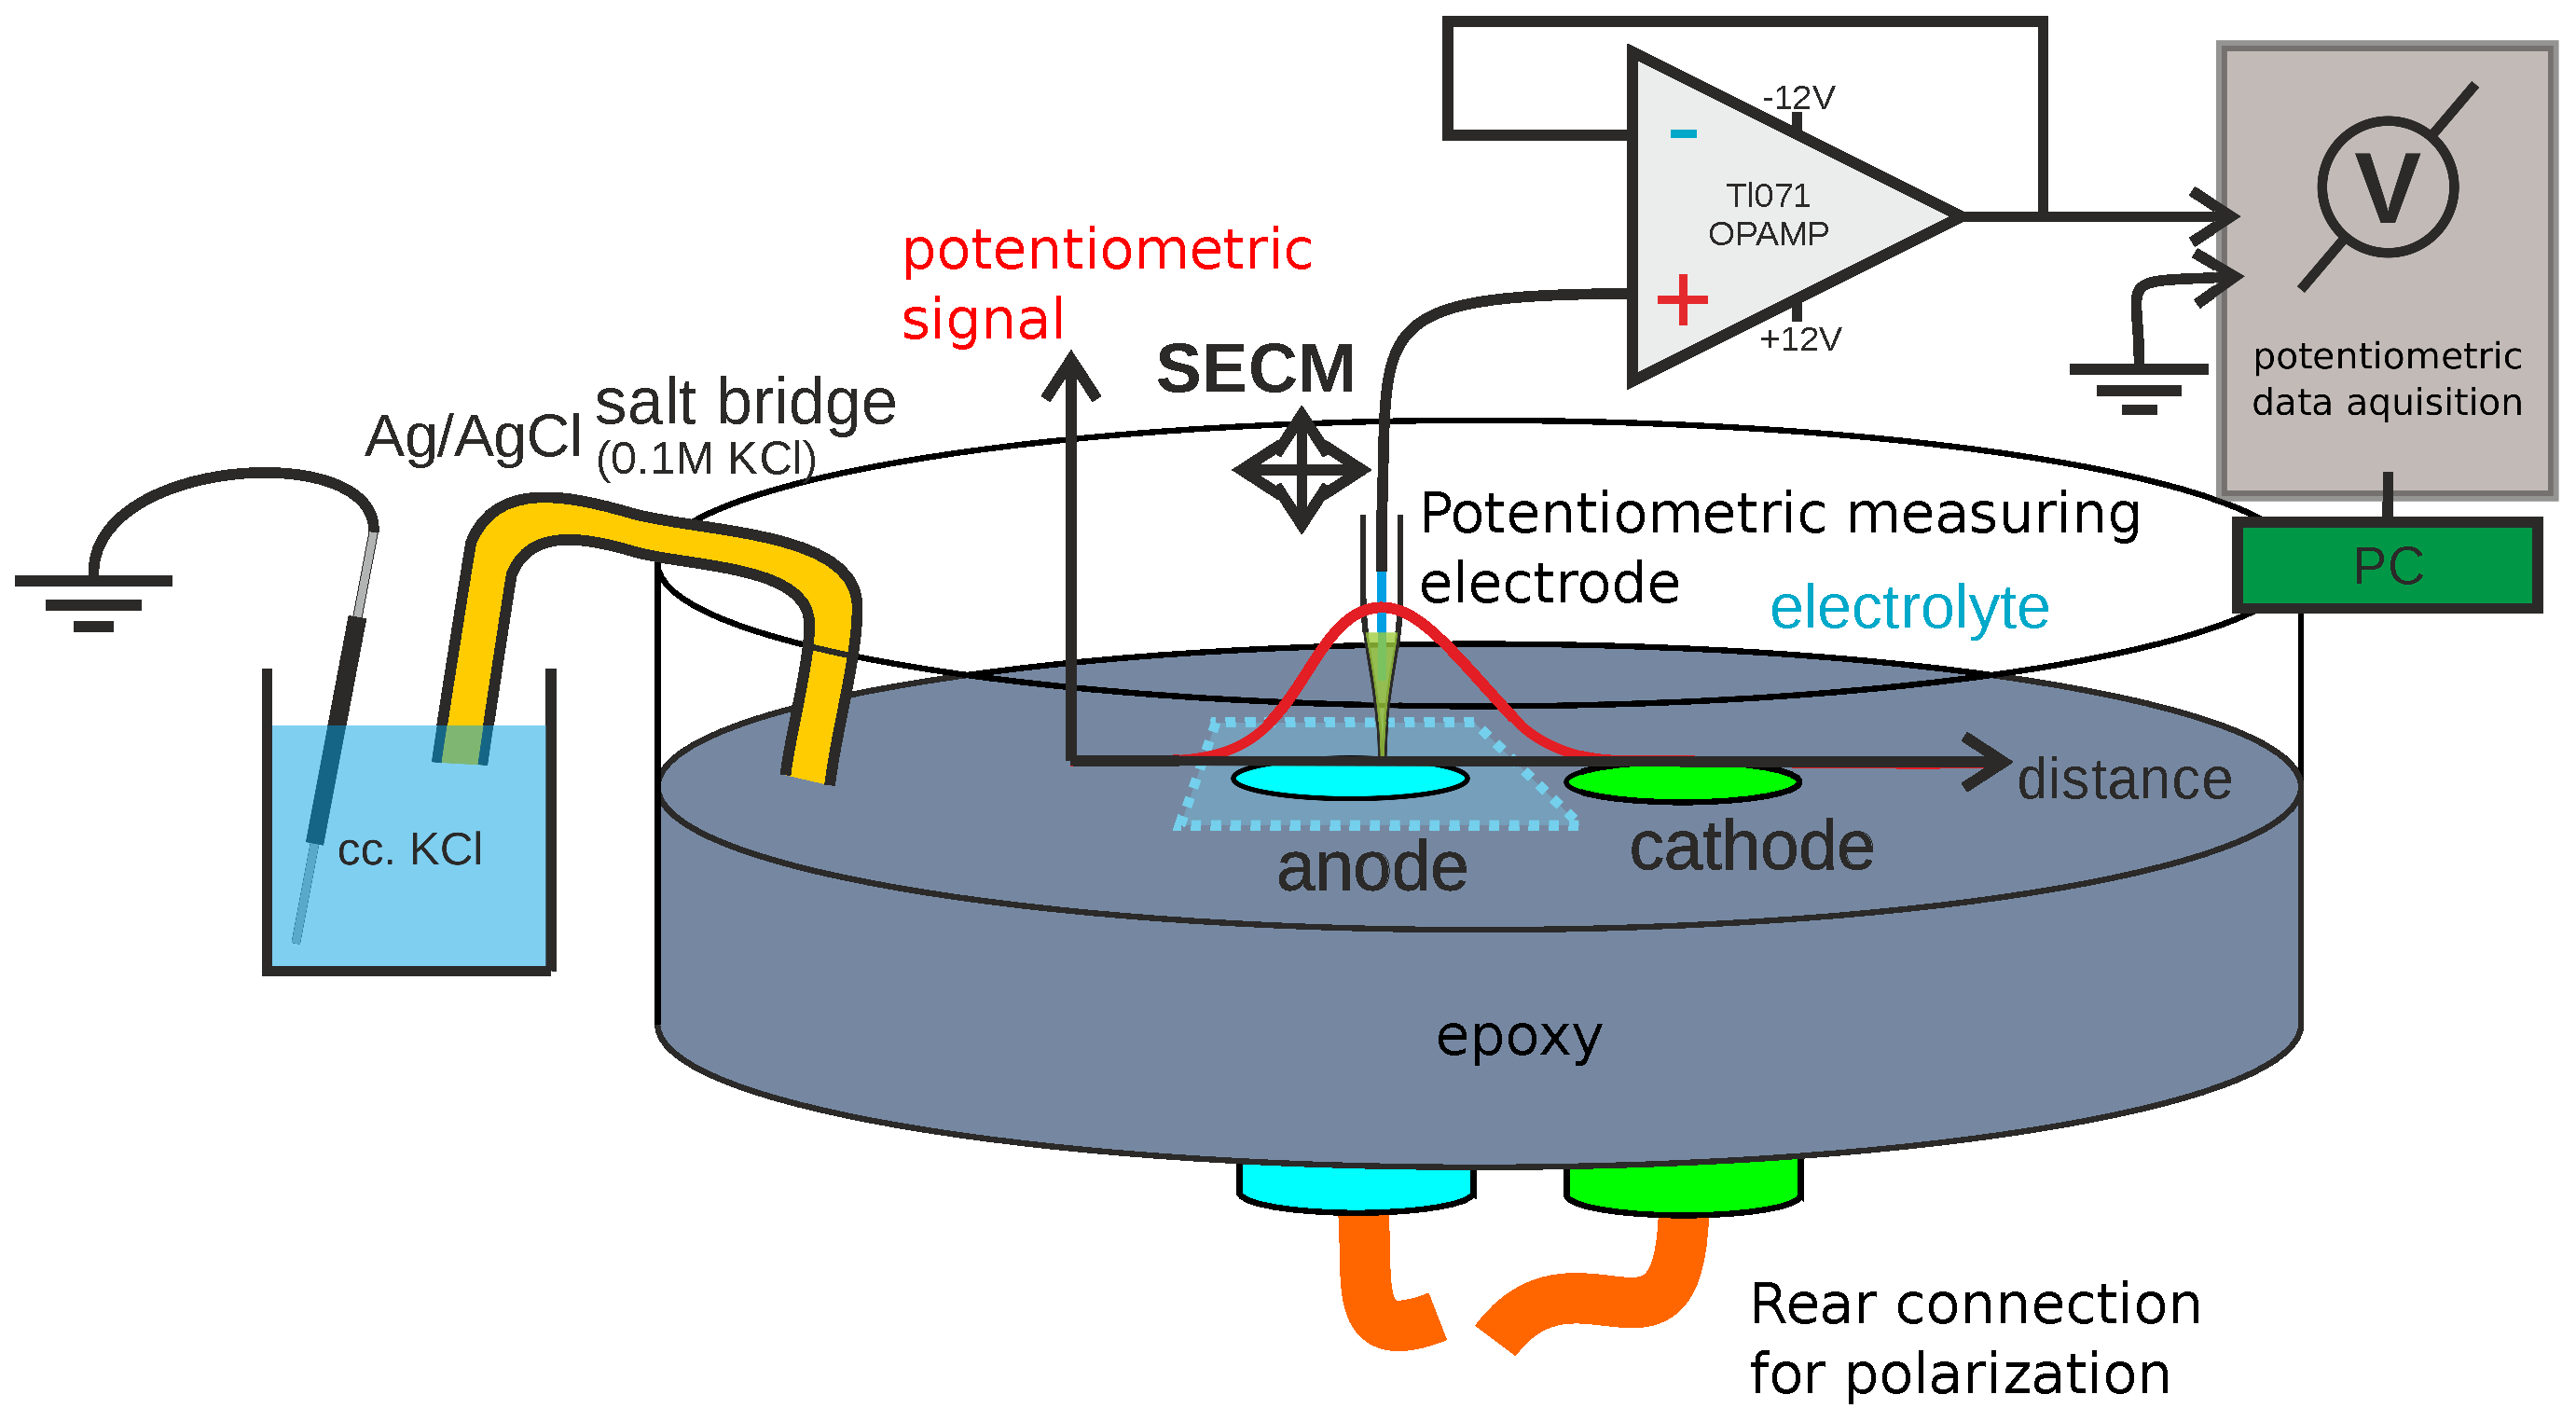
\includegraphics[width=0.9\textwidth]{model.eps}
\end{center}
\end{frame}

\begin{frame}
	\frametitle{Application in corrosion science: galvanic corrosion of Mg} 
	\framesubtitle{Results}
	\centering
	\quad\quad\quad\quad Liquid contact \hfill Solid contact \quad\quad\quad\quad\quad

	\includegraphics[trim = 10mm 30mm 0mm 20mm, clip, width=0.4\textwidth, angle=-90]{liquid_coupled.eps}\includegraphics[trim = 10mm 30mm 0mm 20mm, clip, width=0.4\textwidth, angle=-90]{solid_coupled.eps}
\end{frame}



\begin{frame} [plain]
\centering
Solution \#2:
Optimizing scanning patterns and algorithms.
\end{frame}

\begin{frame}
	\frametitle{New SECM scanning patterns based on the polar-coordinate system}
	\centering	
	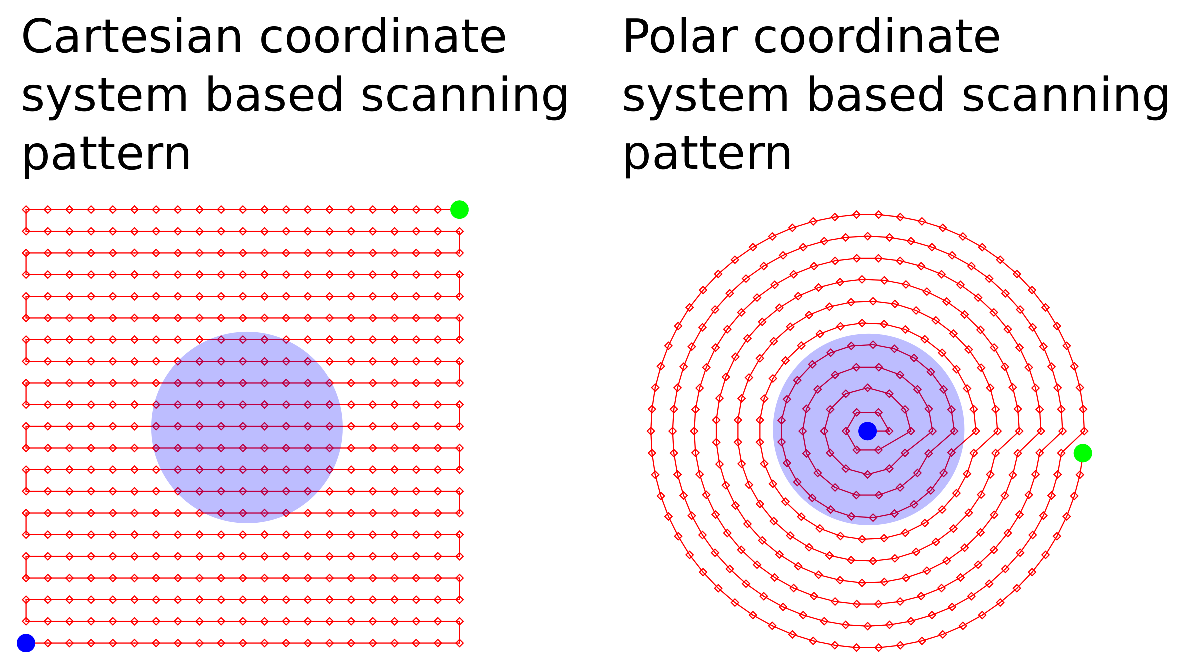
\includegraphics[width=0.7\textwidth]{cartesian_vs_polar.eps}
	
	\vfill
\end{frame}

\begin{frame}
	\frametitle{Simulated SECM scans}	
	\framesubtitle{Using the Cartesian and the polar coordinate system based algorithms}
	\centering
	\includegraphics[width=0.3\textwidth, angle=-90]{meander_sim.eps}\includegraphics[width=0.3\textwidth, angle=-90]{arc_sim.eps}
	\vfill
\end{frame}


\begin{frame}
	\frametitle{Comparison of the simulated scans}
%Parameters of the simulations:\\
%\begin{itemize}
%\item 2000 $\upmu$m $\times$ 2000 $\upmu$m scan area,
%\item 100 $\upmu$m $\times$ 100 $\upmu$m resolution,
%\item 1 s for each data aquisition point,
%\item 500 $\upmu$m/s probe positioning speed.
%\end{itemize}

%\vfill
\begin{table}
		\label{table:comp}
		\centering
		\begin{tabular}{r c c c}
			Algorithm & n & time (s) & mean squared error \\
			\hline
			Meander & 441 & 440 & \textcolor{white!100}{\colorbox{red!100}{$2.75\times 10^{-2}$}} \\
			Fast comb& 441 & 520  & \colorbox{white}{$2.07\times 10^{-2}$} \\
			Comb & 441 & 881 & \colorbox{white}{$2.75\times 10^{-2}$} \\
			Web & 110 & 109 & \colorbox{white}{$9.63\times 10^{-3}$} \\
			Arc & 341 & 340 & \colorbox{green!100}{$2.95\times 10^{-3}$} \\
		\end{tabular}
\end{table}
\end{frame}

\begin{frame}
\frametitle{Confirmation with experimental SECM scans}
\framesubtitle{Antimony microelectrode as pH sensor}
\centering
\begin{equation*}
    \ce{2Sb + 3H_2O <=> Sb_2O_3 + 6H^+ + 6e^-}
\end{equation*}
\includegraphics[width=0.7\textwidth]{antimony.eps}

%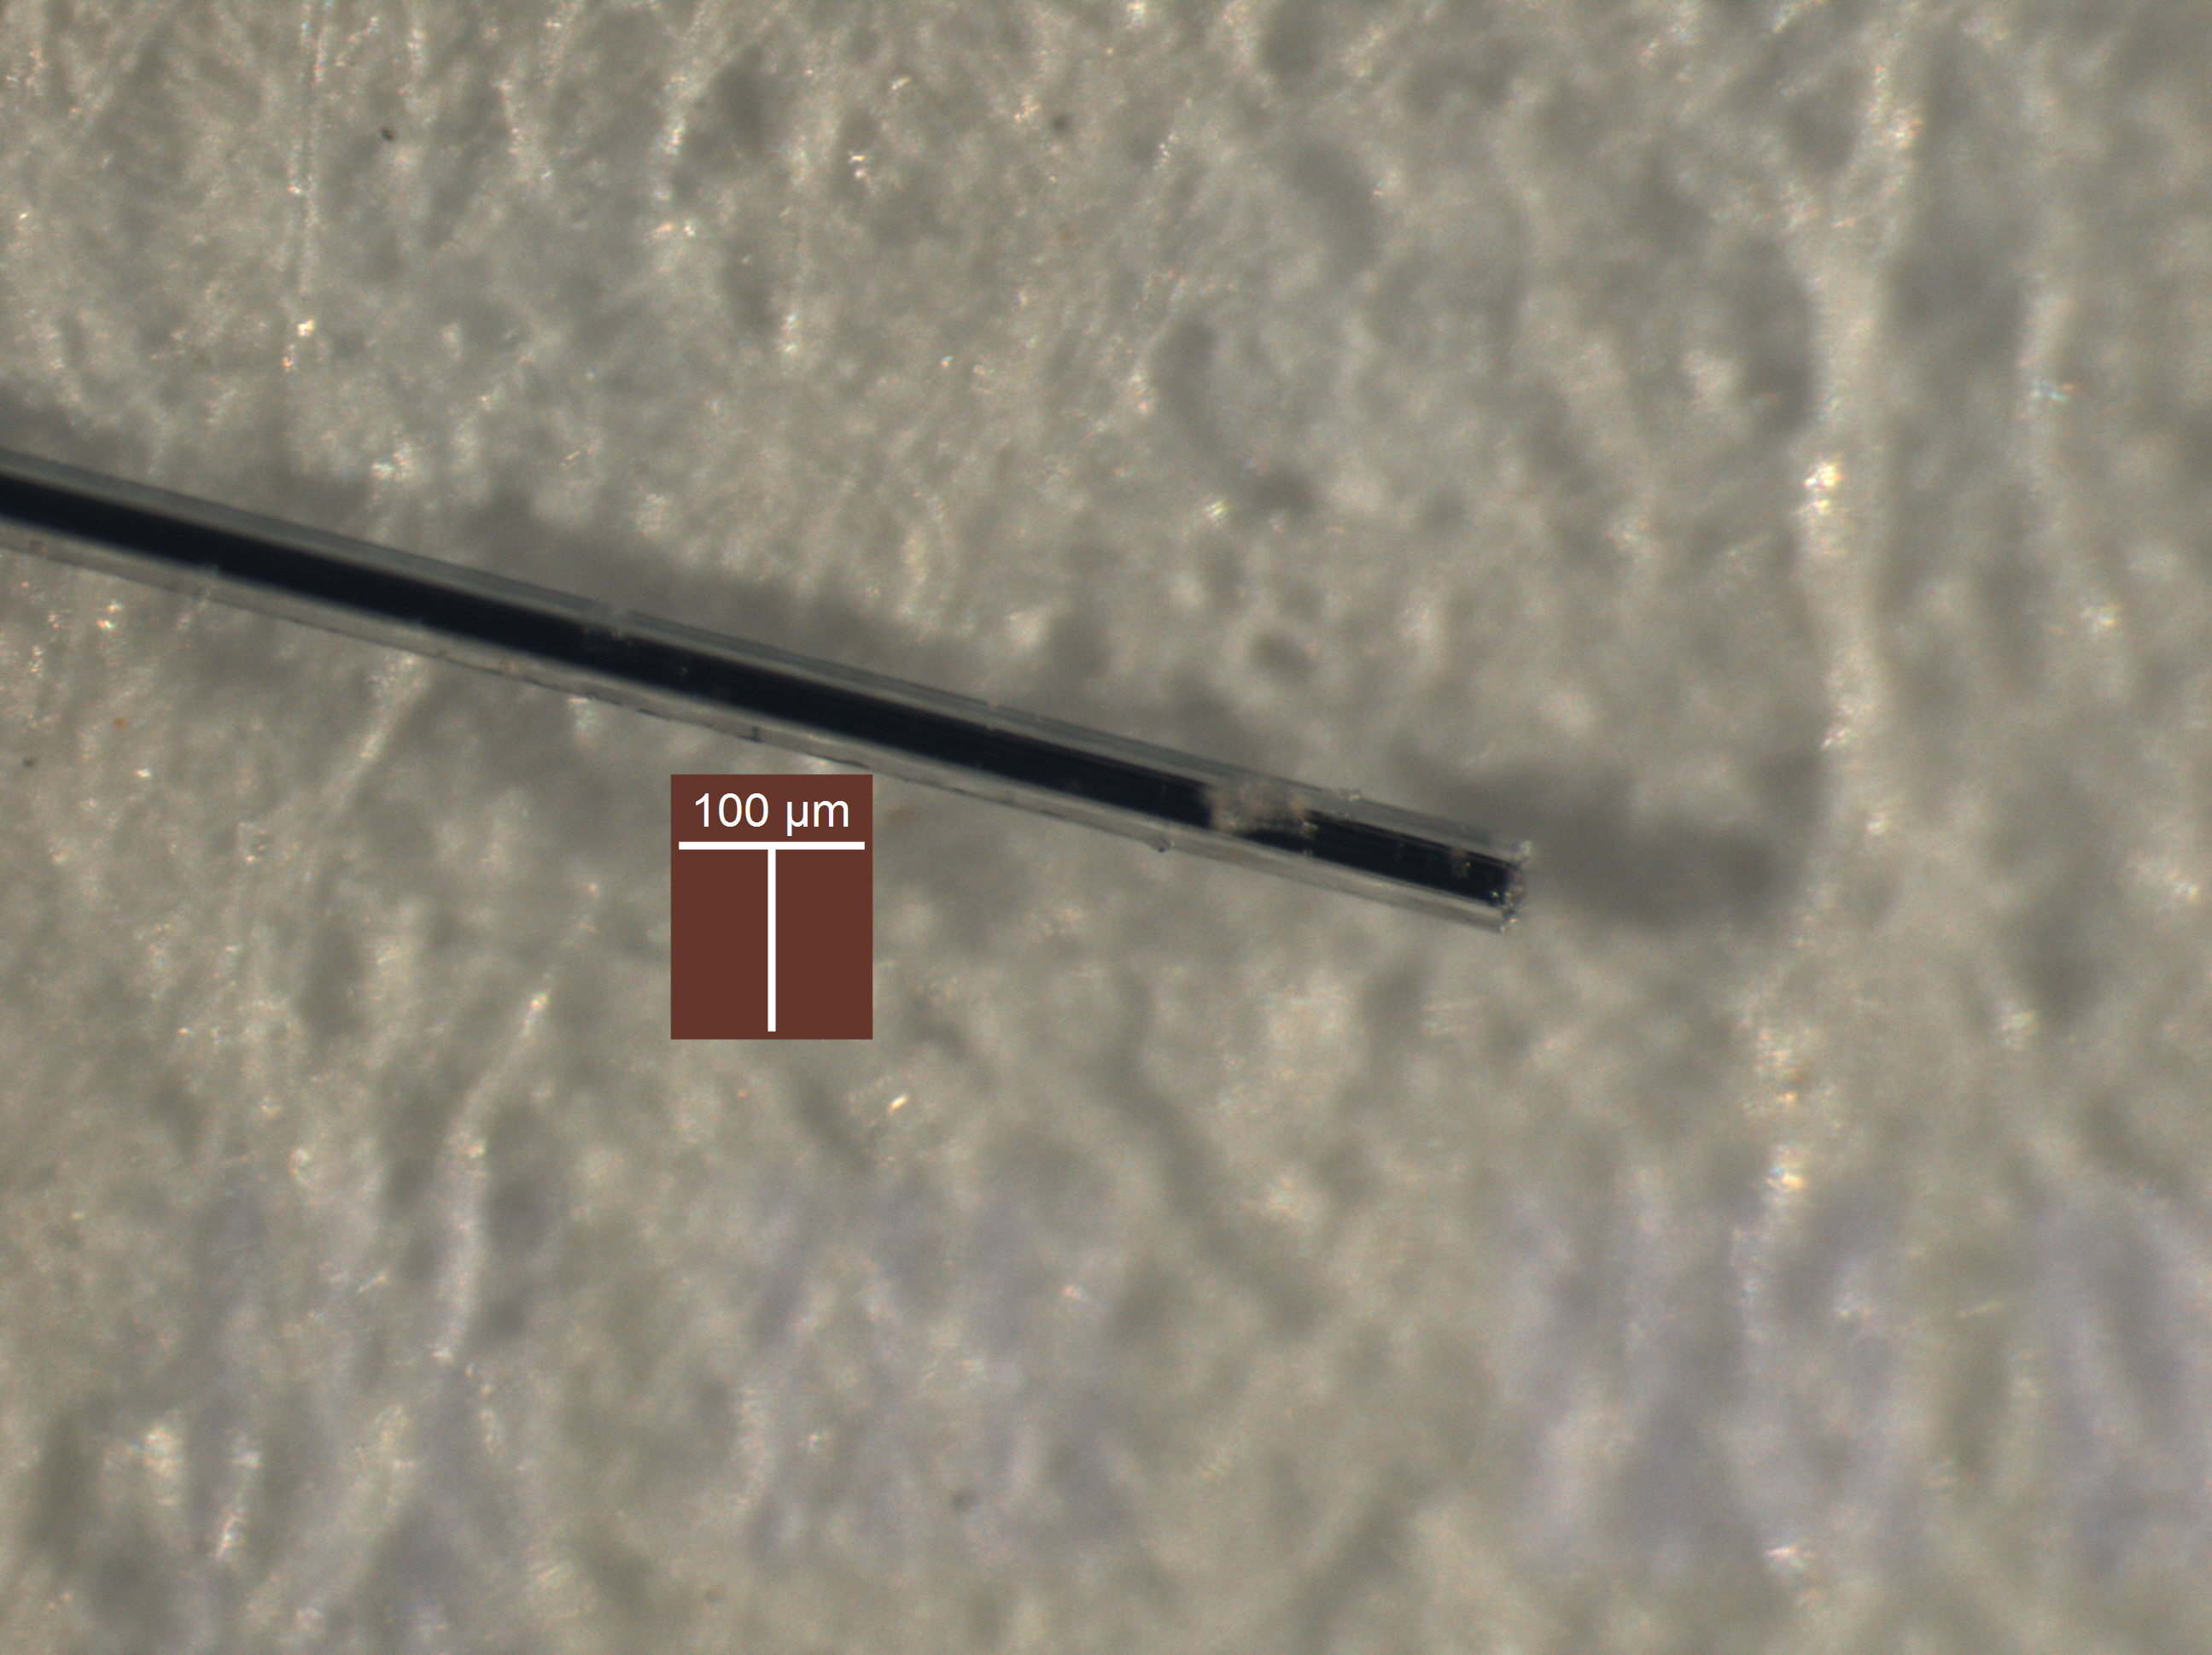
\includegraphics[width=0.4\textwidth]{sb.jpg}
\end{frame} 


\begin{frame}
	\centering
	\frametitle{Confirmation with experimental SECM scans}
	\framesubtitle{Recorded using the antimony microelectrode}
	\includegraphics[width=0.3\textwidth, angle=-90]{meander.eps}\includegraphics[width=0.3\textwidth, angle=-90]{arc.eps}\\
	\vfill
	Scans are completed almost 2 times faster,\\ images have almost 10 times less distortion.
\end{frame}

\begin{frame}[plain]
\centering
Solution \#3: Signal processing.
\end{frame}

\begin{frame}
\frametitle{The convolution function of the distortion}
\centering	
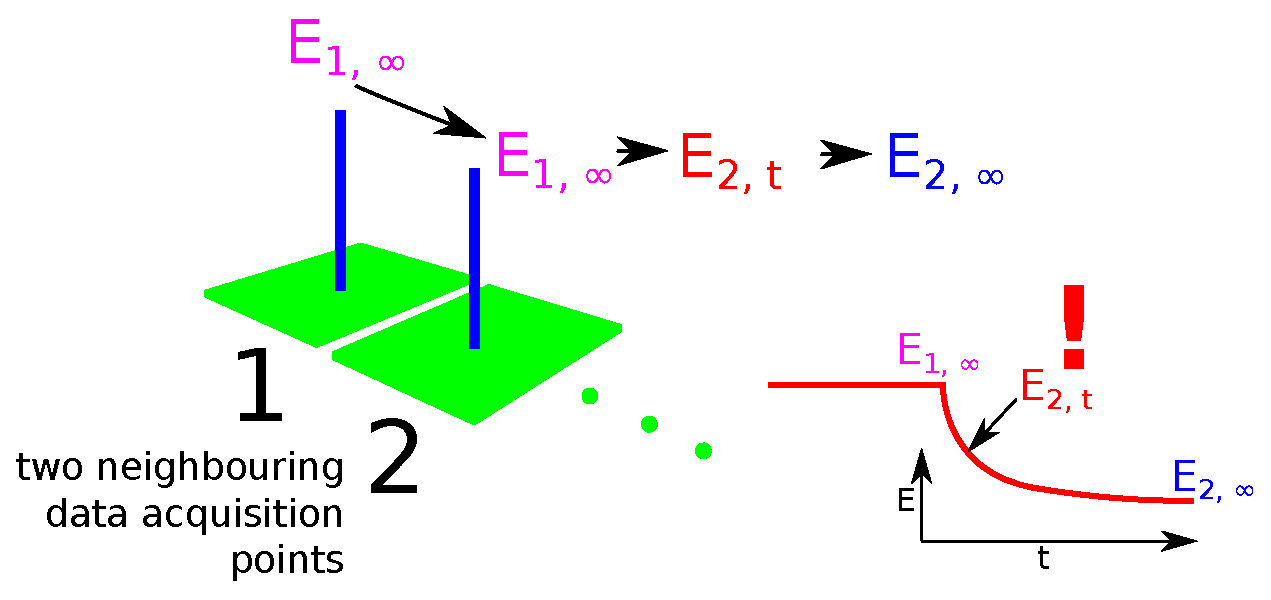
\includegraphics[width=1\textwidth]{t.eps}\\
\vfill
$E_{cell}(t) = E_{cell}(\infty) + [E_{cell}(0) - E_{cell}(\infty)]e^{-t/RC}$\\
\vfill
%$E_{cell}(\infty)	= \frac {\displaystyle [E_{cell}(t) - E_{cell}(0)]e^{-t/RC}}	{\displaystyle 1 - e^{-t/RC}}$
\end{frame}

\begin{frame}
\frametitle{Convolution and deconvolution}
\centering
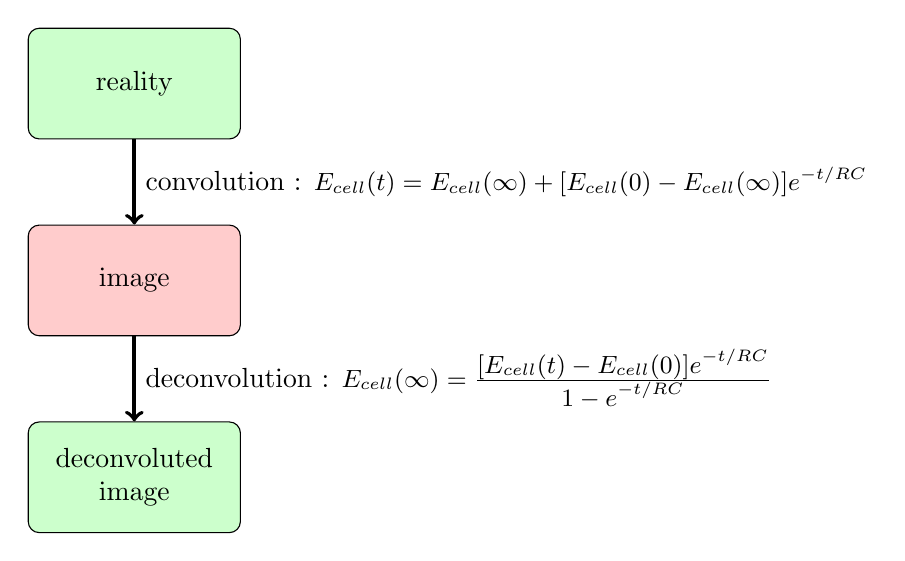
\begin{tikzpicture}[node distance = 2.5cm, auto]
\node [rectangle, draw, fill=green!20,text width=7em, text centered, rounded corners, minimum height=4em] (reality) {reality};
\node [rectangle, below of=reality, draw, fill=red!20,text width=7em, text centered, rounded corners, minimum height=4em] (measurement) {image};
\node [rectangle, below of=measurement, draw, fill=green!20,text width=7em, text centered, rounded corners, minimum height=4em] (image) {deconvoluted\\ image};

\draw [line width=0.5mm, ->] (reality) -- (measurement) node [pos=.5, right] (TextNode) {convolution : \small $E_{cell}(t) = E_{cell}(\infty) + [E_{cell}(0) - E_{cell}(\infty)]e^{-t/RC}$};
\draw [line width=0.5mm, ->] (measurement) -- (image) node [pos=.5, right] (TextNode) {deconvolution : \small $E_{cell}(\infty)      = \frac {\displaystyle [E_{cell}(t) - E_{cell}(0)]e^{-t/RC}}    {\displaystyle 1 - e^{-t/RC}}$};


\end{tikzpicture}
\end{frame}


\begin{frame}
	\frametitle{Deconvolution of potentiometric SECM images}
	\framesubtitle{Recorded using the antimony microelectrode following the meander algorithm}
\centering

\def\s{0.15}

\begin{columns}[T] % align columns

\begin{column}{.2\textwidth}
\begin{minipage}[c][0.75\textheight][c]{\linewidth}
\centering
%raw\\
%images
\end{minipage}
\end{column}%
\hfill%
\begin{column}{.2\textwidth}
\centering
\includegraphics[trim = 10mm 30mm 0mm 10mm, clip, width=0.8\textwidth, angle=-90]{13121313.eps}\\
\includegraphics[trim = 10mm 30mm 0mm 10mm, clip, width=0.8\textwidth, angle=-90]{13121314.eps}\\
\includegraphics[trim = 10mm 30mm 0mm 10mm, clip, width=0.8\textwidth, angle=-90]{13121315.eps}\\
\includegraphics[trim = 10mm 30mm 0mm 10mm, clip, width=0.8\textwidth, angle=-90]{13121316.eps}\\
\end{column}%
\begin{column}{.2\textwidth}
\begin{minipage}[c][0.7\textheight][c]{\linewidth}
\centering
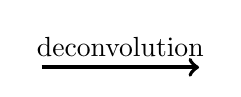
\begin{tikzpicture}
\draw [line width=0.5mm,->] (0,0) -- (2,0) node [pos=.5, above] (TextNode) {deconvolution};
\end{tikzpicture}
\end{minipage}
\end{column}%
\begin{column}{.2\textwidth}
\centering
\includegraphics[trim = 10mm 30mm 0mm 10mm, clip, width=0.8\textwidth, angle=-90]{13121313_deconvoluted.eps}\\
\includegraphics[trim = 10mm 30mm 0mm 10mm, clip, width=0.8\textwidth, angle=-90]{13121314_deconvoluted.eps}\\
\includegraphics[trim = 10mm 30mm 0mm 10mm, clip, width=0.8\textwidth, angle=-90]{13121315_deconvoluted.eps}\\
\includegraphics[trim = 10mm 30mm 0mm 10mm, clip, width=0.8\textwidth, angle=-90]{13121316_deconvoluted.eps}\\
\end{column}%
\begin{column}{.2\textwidth}
\begin{minipage}[c][0.75\textheight][c]{\linewidth}
\centering
%deconvoluted\\
%images
\end{minipage}
\end{column}%
\end{columns}
\end{frame}

\begin{frame}
\begin{center}
\frametitle{Deconvolution of potentiometric SECM images}
\framesubtitle{Recorded using the magnesium ISME following the meander algorithm}
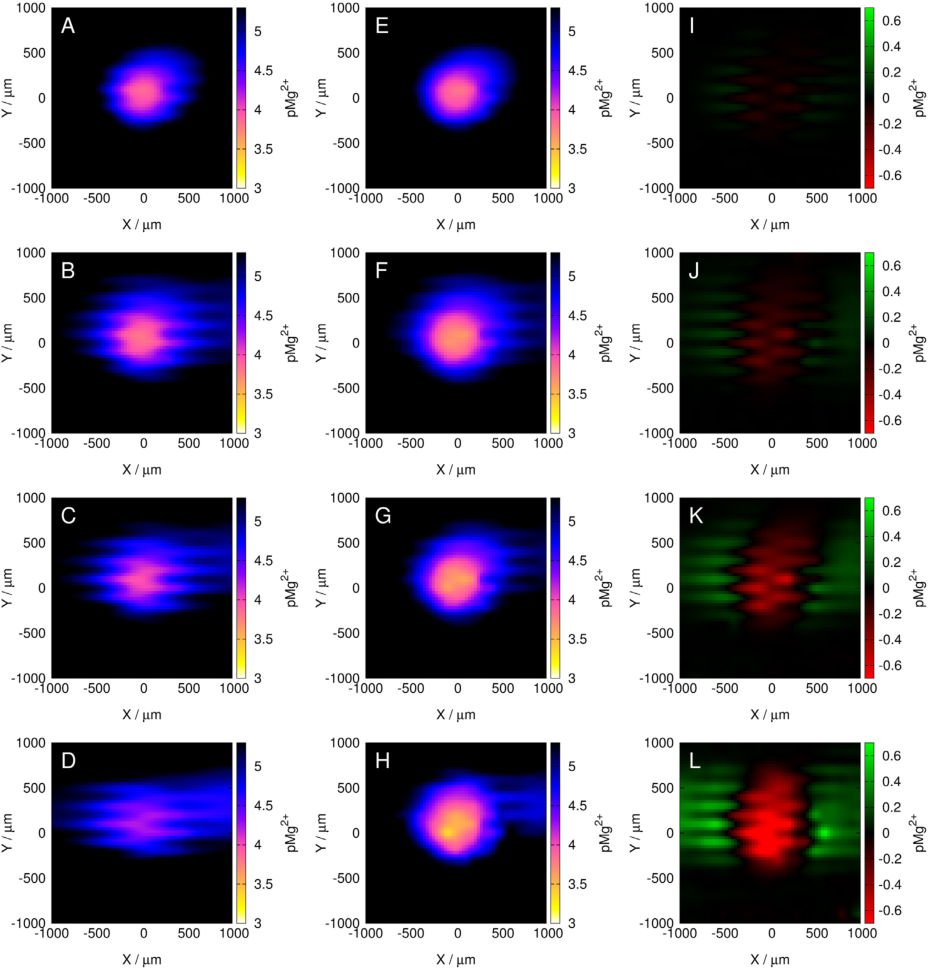
\includegraphics[width=0.6\textwidth]{mg_2d.pdf}
\end{center}
\end{frame}

\begin{frame}
\frametitle{Practical example: corroding carbon steel sample}
\framesubtitle{Scanned with an antimony microelectrode}
\begin{figure}
\centering
%top left bottom right
\includegraphics[trim = 10mm 30mm 0mm 10mm, clip, width=0.3\textwidth, angle=-90]{16012906.eps}\includegraphics[trim = 10mm 30mm 0mm 10mm, clip, width=0.3\textwidth, angle=-90]{16012906_deconvoluted.eps}

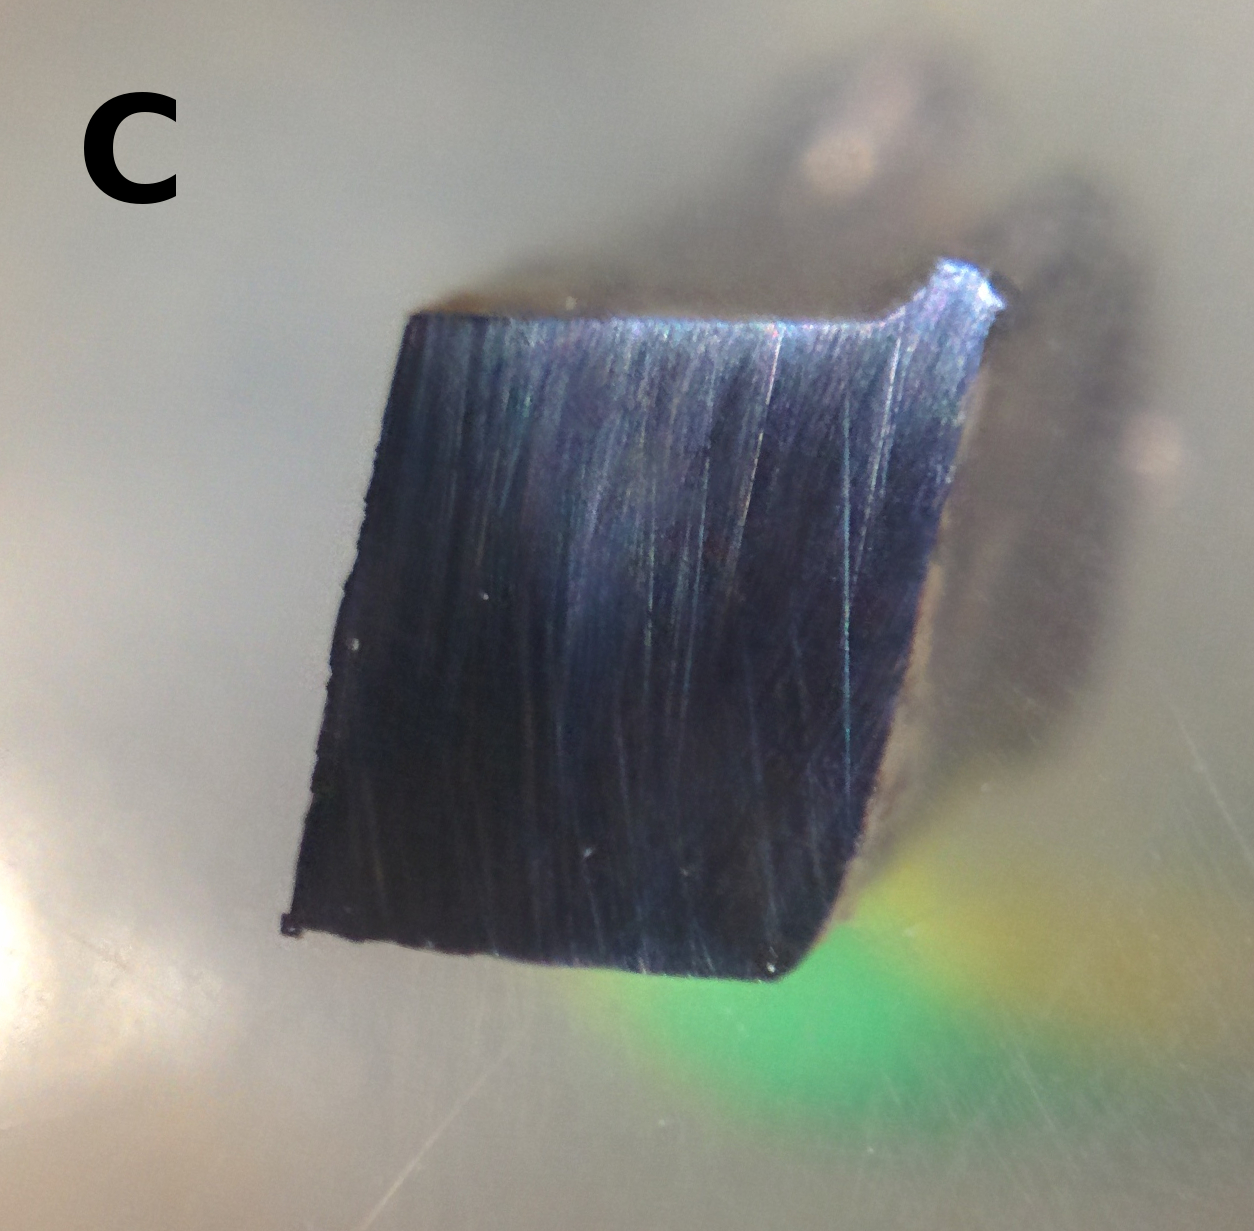
\includegraphics[width=0.24\textwidth]{cs_cut.jpg}

%\caption[Raw, and deconvoluted SECM image and microphoto of a corroding carbon-steel sample polarized anodically.]{Raw (A), and deconvoluted (B) SECM image and microphoto (C) of a corroding carbon-steel sample polarized anodically with a current density of 10 $mA/cm^2$. Measuring electrode was an antimony pH microelectrode. Potential was measured against an Ag/AgCl/3M KCl. Recorded $h$ = 100 $\upmu$m above the surface with probe movement speed of 1000 $\upmu$m/s, equilibration interval 0.4 s.}
\end{figure}
\end{frame}

\begin{frame}[plain]
\centering
The effect of electric field on potentiometric SECM imaging.
\end{frame}

\begin{frame}
\begin{center}
\frametitle{The electric field during galvanic corrosion}
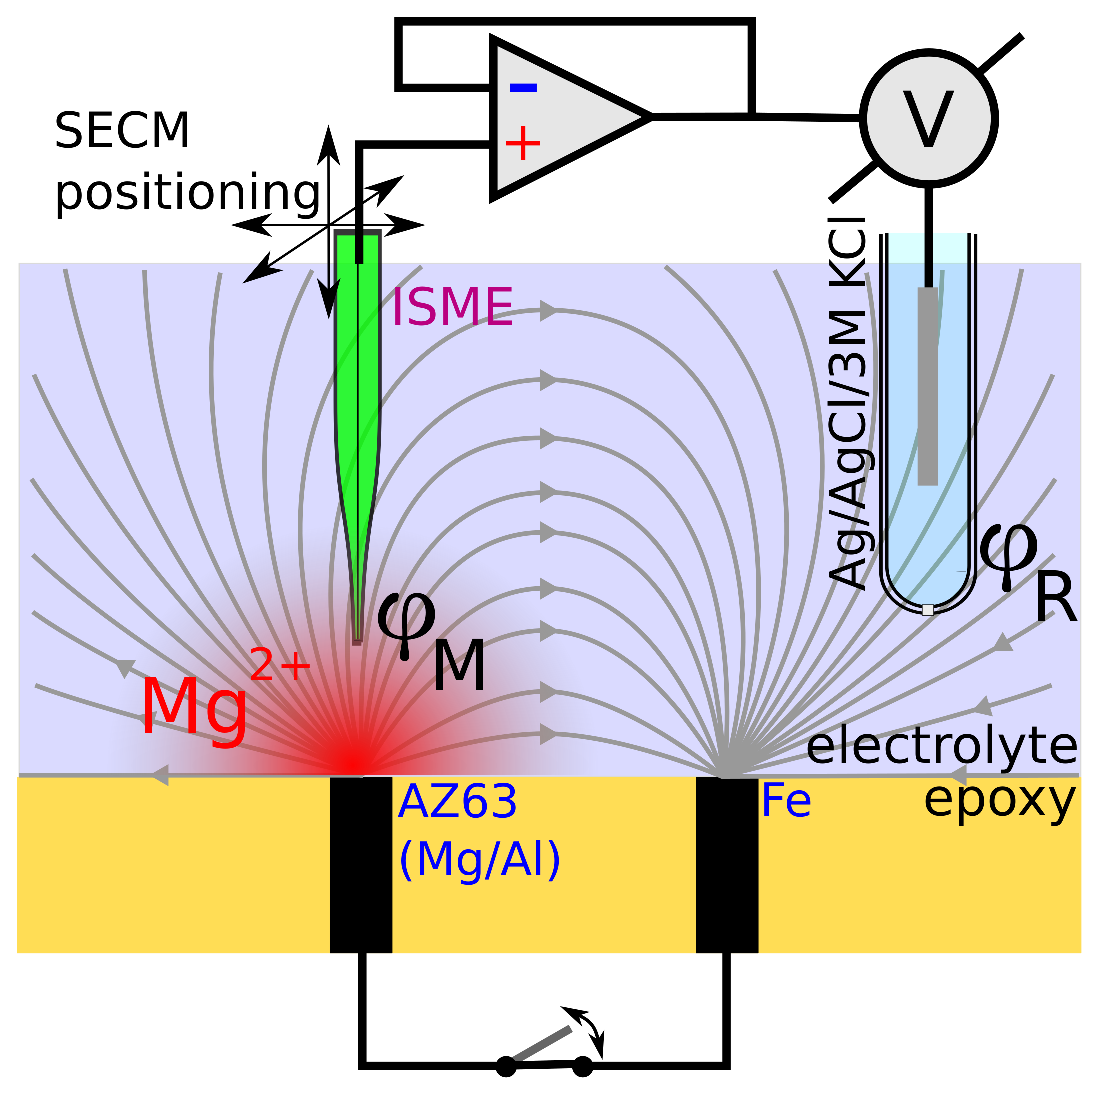
\includegraphics[width=0.5\textwidth]{field.eps}

\begin{equation*}
\Delta E=E_M-E_R + (\phi_M - \phi_R)
\label{eq:potential}
\end{equation*}
\end{center}
\end{frame}

\begin{frame}
\frametitle{The effect of electric field on the measured potential}
\framesubtitle{}
\centering
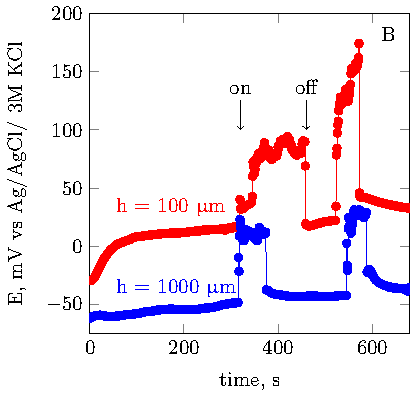
\includegraphics[width=0.466\textwidth]{field-figure1.pdf}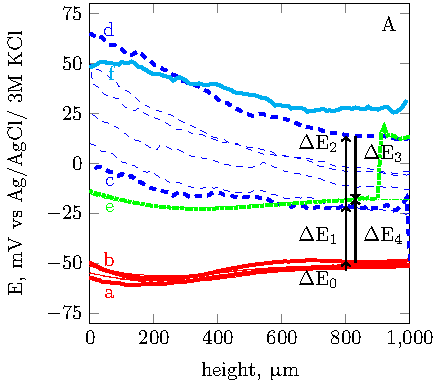
\includegraphics[width=0.5\textwidth]{field-figure0.pdf}
\end{frame}

\begin{frame}
\frametitle{The effect of electric field on potentiometric SECM imaging}
\centering
\includegraphics[trim = 10mm 20mm 0mm 10mm, clip, width=0.36\textwidth, angle=-90]{17012501.eps}\includegraphics[trim = 10mm 20mm 0mm 10mm, clip, width=0.36\textwidth, angle=-90]{17012503_deconvoluted.eps}
\end{frame}

\begin{frame}
\frametitle{Conclusions}
\begin{enumerate}
\item I've successfully shortened the response time of the potentiometric cell by using low resistance, solid-contact microelectrodes.
I've compared them to conventional, liquid contact microelectrodes by basic characterization and model system study to prove the improved performance.

\item Taking adventage of the new solid-contact electrodes, I've studied the galvanic corrosion of magnesium and the AZ63 magnesium alloy by mapping the concentration of dissolving ions.
I used the new solid contact ion selective microelectrodes as SECM probes. This allowed faster scan rates.
\end{enumerate}
\end{frame}

\begin{frame}
\frametitle{Conclusions}
\begin{enumerate}
\setcounter{enumi}{2}
\item I've estimated the corrosion current based on the SECM measurements, and compared the result with that obtained with another, established method; the indirect measurement of corrosion current.
After applying Faraday's Law of Electrolysis, the two results could be compared.
They were very similar, suggesting the applicability of SECM in obtaining quantitative results.

\item I've designed new scanning patterns and algorithms, optimized to radially symmetric targets.
I've proven that with these new patterns and algorithms, image distortion is lower compared to the conventional ones, by numerical simulations and experimental SECM scans.
\end{enumerate}
\end{frame}

\begin{frame}
\frametitle{Conclusions}
\begin{enumerate}
\setcounter{enumi}{4}
\item I've shown that by using deconvolution, \emph{RC} distortion can be significantly lowered in the potentiometric SECM images.
To prove the validity of the technique, I've compared deconvoluted images to equilibrium images scanned at a rate which allowed to record equilibrium potentials.

\item I've used deconvolution to restore potentiometric SECM images about a corroding carbon steel sample.
Evaluation of this data was possible, because scanning time \emph{and} distortion was reduced at the same time.

\item I've shown the applicability of blind deconvolution.
This method can be used on measurements where the convolution function cannot be determined.
\end{enumerate}
\end{frame}

\begin{frame}
\frametitle{Conclusions}
\begin{enumerate}
\setcounter{enumi}{7}
\item I've proven that the electric field present in many studied systems -- galvanically corroding ones in particular -- affects the measured potential.
The electric field has a direct influence on the measured potential, which is then a sum of this contribution and the Nernstian response associated with ion activity.
This effect can cause serious errors in interpretations in the measurements.
In this case, the error was almost four orders of magnitude.
By taking this effect into account, a more accurate conclusion can be drawn.
\end{enumerate}
\end{frame}

\begin{frame}
	\frametitle{Acknowledgements}
\end{frame}

\end{document}
